% *************************************************************************************************************************
% *************************************         MATEMATICAS DISCRETAS         *********************************************
% *************************************************************************************************************************


% =======================================================
% =======         HEADER FOR DOCUMENT        ============
% =======================================================
    
    % *********  SPECIFIC FOR THIS BOOK  ********
    \def\ProjectAuthorLink{https://github.com/CompilandoConocimiento}
    \def\ProjectNameLink{\ProjectAuthorLink/LibroMatematicasDiscretas}    
    

    % *********   DOCUMENT ITSELF   **************
    \documentclass[12pt, fleqn]{report}                             %Type of doc and size of font and left equations
    \usepackage[margin=1.2in]{geometry}                             %Margins and Geometry pacakge
    \usepackage{ifthen}                                             %Allow simple programming using if - then
    \usepackage[hidelinks]{hyperref}                                %Allow to create hiperlinks and Fuck Firefox
    \usepackage{pdfpages}                                           %Allow us 'import' PDF's
    \hypersetup{pageanchor=false}                                   %Solve 'double page 1' warnings in build :v
    \setlength{\parindent}{0pt}                                     %Eliminate ugly indentation
    \author{Oscar Andrés Rosas}                                     %Who I am

    % *********   LANGUAJE    *****************
    \usepackage[spanish]{babel}                                     %Please allow me to type in spanish
    \usepackage[utf8]{inputenc}                                     %Lets use UFT-8
    \usepackage[T1]{fontenc}                                        %Allow for better font support
    \usepackage{textcmds}                                           %Allow us to use quoutes
    \usepackage{changepage}                                         %Allow us to use identate paragraphs
    \usepackage{anyfontsize}                                        %All the sizes for fonts wiiiii!

    % *********   MATH AND HIS STYLE  *********
    \usepackage{ntheorem, amsmath, amssymb, amsfonts}               %All fucking math, I want all!
    \usepackage{mathrsfs, mathtools, empheq}                        %All fucking math, I want all!
    \usepackage{cancel}                                             %Negate symbol
    \usepackage{centernot}                                          %Allow me to negate a symbol
    \decimalpoint                                                   %Use decimal point

    % *********   GRAPHICS AND IMAGES *********
    \usepackage{graphicx}                                           %Allow to create graphics
    \usepackage{float}                                              %For images
    \usepackage{wrapfig}                                            %Allow to create images
    \graphicspath{ {Graphics/} }                                    %Where are the images :D

    % *********   LISTS AND TABLES ***********
    \usepackage{listings, listingsutf8}                             %We will be using code here
    \usepackage[inline]{enumitem}                                   %We will need to enumarate
    \usepackage{tasks}                                              %Horizontal lists
    \usepackage{longtable}                                          %Lets make tables awesome
    \usepackage{booktabs}                                           %Lets make tables awesome
    \usepackage{tabularx}                                           %Lets make tables awesome
    \usepackage{multirow}                                           %Lets make tables awesome
    \usepackage{multicol}                                           %Create multicolumns

    % *********   REMOVE SOME ERRORS **********
    \hbadness=10000                                                 %Ignore \vbox and \hbox warings
    \hfuzz=\maxdimen\newdimen\hfuzz                                 %Ignore \vbox and \hbox warings

    % *********   HEADERS AND FOOTERS ********
    \usepackage{fancyhdr}                                           %Lets make awesome headers/footers
    \pagestyle{fancy}                                               %Lets make awesome headers/footers
    \setlength{\headheight}{16pt}                                   %Top line
    \setlength{\parskip}{0.5em}                                     %Top line
    \renewcommand{\footrulewidth}{0.5pt}                            %Bottom line

    \lhead {                                                        %Left Header
        \hyperlink{chapter.\arabic{chapter}}                        %Make a link to the current chapter
        {\normalsize{\textsc{\nouppercase{\leftmark}}}}             %And fot it put the name
    }

    \rhead {                                                        %Right Header
        \hyperlink{section.\arabic{chapter}.\arabic{section}}       %Make a link to the current chapter
            {\footnotesize{\textsc{\nouppercase{\rightmark}}}}      %And fot it put the name
    }

    \rfoot{\textsc{\small{\hyperref[sec:Index]{Ve al Índice}}}}     %This will always be a footer  

    \fancyfoot[L]{                                                  %Algoritm for a changing footer
        \ifthenelse{\isodd{\value{page}}}                           %IF ODD PAGE:
            {\href{https://SoyOscarRH.github.io/}                   %DO THIS:
                {\footnotesize                                      %Send the page
                    {\textsc{Oscar Andrés Rosas}}}}                 %Send the page
            {\href{https://compilandoconocimiento.com}              %ELSE DO THIS: 
                {\footnotesize                                      %Send the author
                    {\textsc{Compilando Conocimiento}}}}            %Send the author
    }
    
    
% =======================================================
% ===================   COMMANDS    =====================
% =======================================================

    % =========================================
    % =======   NEW ENVIRONMENTS   ============
    % =========================================
    \newenvironment{Indentation}[1][0.75em]                         %Use: \begin{Inde...}[Num]...\end{Inde...}
        {\begin{adjustwidth}{#1}{}}                                 %If you dont put nothing i will use 0.75 em
        {\end{adjustwidth}}                                         %This indentate a paragraph
    
    \newenvironment{SmallIndentation}[1][0.75em]                    %Use: The same that we upper one, just 
        {\begin{adjustwidth}{#1}{}\begin{footnotesize}}             %footnotesize size of letter by default
        {\end{footnotesize}\end{adjustwidth}}                       %that's it
    
    \def \Eq {equation}                                             %Stupid Visual studio error
    \newenvironment{MultiLineEquation}[1]                           %Use: To create MultiLine equations
        {\begin{\Eq}\begin{alignedat}{#1}}                          %Use: \begin{Multi..}{Num. de Columnas}
        {\end{alignedat}\end{\Eq}}                                  %And.. that's it!
    
    \newenvironment{MultiLineEquation*}[1]                          %Use: To create MultiLine equations
        {\begin{\Eq*}\begin{alignedat}{#1}}                         %Use: \begin{Multi..}{Num. de Columnas}
        {\end{alignedat}\end{\Eq*}}                                 %And.. that's it!
    

    % =========================================
    % == GENERAL TEXT & SYMBOLS ENVIRONMENTS ==
    % =========================================
    
    % =====  TEXT  ======================
    \newcommand \Quote              {\qq}                           %Use: \Quote to use quotes
    \newcommand \Over               {\overline}                     %Use: \Bar to use just for short
    \newcommand \ForceNewLine       {$\Space$\\}                    %Use it in theorems for example
    \newcommand \ForceColumnBreak   {\vfill\null\columnbreak}       %Use only in multicols

    % =====  SPACES  ====================
    \DeclareMathOperator \Space     {\quad}                         %Use: \Space for a cool mega space
    \DeclareMathOperator \MegaSpace {\quad \quad}                   %Use: \MegaSpace for a cool mega mega space
    \DeclareMathOperator \MiniSpace {\;}                            %Use: \Space for a cool mini space
    
    % =====  MATH TEXT  =================
    \newcommand \Such           {\MiniSpace | \MiniSpace}           %Use: \Such like in sets
    \newcommand \Also           {\MiniSpace \text{y} \MiniSpace}    %Use: \Also so it's look cool
    \newcommand \Remember[1]    {\Space\text{\scriptsize{#1}}}      %Use: \Remember so it's look cool
    
    % =====  THEOREMS: IN SPANISH :0  ===
    \newtheorem{Theorem}        {Teorema}[section]                  %Use: \begin{Theorem}[Name]\label{Nombre}...
    \newtheorem{Corollary}      {Colorario}[Theorem]                %Use: \begin{Corollary}[Name]\label{Nombre}...
    \newtheorem{Lemma}[Theorem] {Lemma}                             %Use: \begin{Lemma}[Name]\label{Nombre}...
    \newtheorem{Definition}     {Definición}[section]               %Use: \begin{Definition}[Name]\label{Nombre}...
    \theoremstyle{break}                                            %THEOREMS START 1 SPACE AFTER Fuck!

    % =====  LOGIC  =====================
    \newcommand \lIff    {\leftrightarrow}                          %Use: \lIff for logic iff
    \newcommand \lEqual  {\MiniSpace \Leftrightarrow \MiniSpace}    %Use: \lEqual for a logic double arrow
    \newcommand \lInfire {\MiniSpace \Rightarrow \MiniSpace}        %Use: \lInfire for a logic infire
    \newcommand \lLongTo {\longrightarrow}                          %Use: \lLongTo for a long arrow

    % =====  FAMOUS SETS  ===============
    \DeclareMathOperator \Naturals     {\mathbb{N}}                 %Use: \Naturals por Notation
    \DeclareMathOperator \Primes       {\mathbb{P}}                 %Use: \Primes por Notation
    \DeclareMathOperator \Integers     {\mathbb{Z}}                 %Use: \Integers por Notation
    \DeclareMathOperator \Racionals    {\mathbb{Q}}                 %Use: \Racionals por Notation
    \DeclareMathOperator \Reals        {\mathbb{R}}                 %Use: \Reals por Notation
    \DeclareMathOperator \Complexs     {\mathbb{C}}                 %Use: \Complex por Notation
    \DeclareMathOperator \GenericField {\mathbb{F}}                 %Use: \GenericField por Notation
    \DeclareMathOperator \VectorSet    {\mathbb{V}}                 %Use: \VectorSet por Notation
    \DeclareMathOperator \SubVectorSet {\mathbb{W}}                 %Use: \SubVectorSet por Notation
    \DeclareMathOperator \Polynomials  {\mathbb{P}}                 %Use: \Polynomials por Notation
    \DeclareMathOperator \VectorSpace  {\VectorSet_{\GenericField}} %Use: \VectorSpace por Notation
    \DeclareMathOperator \LinealTransformation {\mathcal{T}}        %Use: \LinealTransformation for a cool T
    \DeclareMathOperator \LinTrans      {\mathcal{T}}               %Use: \LinTrans for a cool T
    \DeclareMathOperator \Laplace       {\mathcal{L}}               %Use: \LinTrans for a cool T

    % =====  CONTAINERS   ===============
    \newcommand{\Set}[1]            {\left\{ \; #1 \; \right\}}     %Use: \Set {Info} for INTELLIGENT space 
    \newcommand{\bigSet}[1]         {\big\{  \; #1 \; \big\}}       %Use: \bigSet  {Info} for space 
    \newcommand{\BigSet}[1]         {\Big\{  \; #1 \; \Big\}}       %Use: \BigSet  {Info} for space 
    \newcommand{\biggSet}[1]        {\bigg\{ \; #1 \; \bigg\}}      %Use: \biggSet {Info} for space 
    \newcommand{\BiggSet}[1]        {\Bigg\{ \; #1 \; \Bigg\}}      %Use: \BiggSet {Info} for space 
        
    \newcommand{\Wrap}[1]           {\left( #1 \right)}             %Use: \Wrap {Info} for INTELLIGENT space
    \newcommand{\bigWrap}[1]        {\big( \; #1 \; \big)}          %Use: \bigBrackets  {Info} for space 
    \newcommand{\BigWrap}[1]        {\Big( \; #1 \; \Big)}          %Use: \BigBrackets  {Info} for space 
    \newcommand{\biggWrap}[1]       {\bigg( \; #1 \; \bigg)}        %Use: \biggBrackets {Info} for space 
    \newcommand{\BiggWrap}[1]       {\Bigg( \; #1 \; \Bigg)}        %Use: \BiggBrackets {Info} for space 

    \newcommand{\Brackets}[1]       {\left[ #1 \right]}             %Use: \Brackets {Info} for INTELLIGENT space
    \newcommand{\bigBrackets}[1]    {\big[ \; #1 \; \big]}          %Use: \bigBrackets  {Info} for space 
    \newcommand{\BigBrackets}[1]    {\Big[ \; #1 \; \Big]}          %Use: \BigBrackets  {Info} for space 
    \newcommand{\biggBrackets}[1]   {\bigg[ \; #1 \; \bigg]}        %Use: \biggBrackets {Info} for space 
    \newcommand{\BiggBrackets}[1]   {\Bigg[ \; #1 \; \Bigg]}        %Use: \BiggBrackets {Info} for space 

    \newcommand{\Generate}[1]   {\left\langle #1 \right\rangle}     %Use: \Generate {Info} <>
    \newcommand{\Floor}[1]      {\left \lfloor #1 \right \rfloor}   %Use: \Floor {Info} for floor 
    \newcommand{\Ceil}[1]       {\left \lceil #1 \right \rceil }    %Use: \Ceil {Info} for ceil
    
    % =====  BETTERS MATH COMMANDS   =====
    \newcommand{\pfrac}[2]      {\Wrap{\dfrac{#1}{#2}}}             %Use: Put fractions in parentesis

    % =========================================
    % ====   LINEAL ALGEBRA & VECTORS    ======
    % =========================================

    % ===== UNIT VECTORS  ================
    \newcommand{\hati}      {\hat{\imath}}                           %Use: \hati for unit vector    
    \newcommand{\hatj}      {\hat{\jmath}}                           %Use: \hatj for unit vector    
    \newcommand{\hatk}      {\hat{k}}                                %Use: \hatk for unit vector

    % ===== MAGNITUDE  ===================
    \newcommand{\abs}[1]    {\left\lvert #1 \right\lvert}           %Use: \abs{expression} for |x|
    \newcommand{\Abs}[1]    {\left\lVert #1 \right\lVert}           %Use: \Abs{expression} for ||x||
    \newcommand{\Mag}[1]    {\left| #1 \right|}                     %Use: \Mag {Info} 
    
    \newcommand{\bVec}[1]   {\mathbf{#1}}                           %Use for bold type of vector
    \newcommand{\lVec}[1]   {\overrightarrow{#1}}                   %Use for a long arrow over a vector
    \newcommand{\uVec}[1]   {\mathbf{\hat{#1}}}                     %Use: Unitary Vector Example: $\uVec{i}

    % ===== FN LINEAL TRANSFORMATION  ====
    \newcommand{\FnLinTrans}[1]{\mathcal{T}\Wrap{#1}}               %Use: \FnLinTrans for a cool T
    \newcommand{\VecLinTrans}[1]{\mathcal{T}\pVector{#1}}           %Use: \LinTrans for a cool T
    \newcommand{\FnLinealTransformation}[1]{\mathcal{T}\Wrap{#1}}   %Use: \FnLinealTransformation

    % ===== ALL FOR DOT PRODUCT  =========
    \makeatletter                                                   %WTF! IS THIS
    \newcommand*\dotP{\mathpalette\dotP@{.5}}                       %Use: \dotP for dot product
    \newcommand*\dotP@[2] {\mathbin {                               %WTF! IS THIS            
        \vcenter{\hbox{\scalebox{#2}{$\m@th#1\bullet$}}}}           %WTF! IS THIS
    }                                                               %WTF! IS THIS
    \makeatother                                                    %WTF! IS THIS

    % === WRAPPERS FOR COLUMN VECTOR ===
    \newcommand{\pVector}[1]                                        %Use: \pVector {Matrix Notation} use parentesis
        { \ensuremath{\begin{pmatrix}#1\end{pmatrix}} }             %Example: \pVector{a\\b\\c} or \pVector{a&b&c} 
    \newcommand{\lVector}[1]                                        %Use: \lVector {Matrix Notation} use a abs 
        { \ensuremath{\begin{vmatrix}#1\end{vmatrix}} }             %Example: \lVector{a\\b\\c} or \lVector{a&b&c} 
    \newcommand{\bVector}[1]                                        %Use: \bVector {Matrix Notation} use a brackets 
        { \ensuremath{\begin{bmatrix}#1\end{bmatrix}} }             %Example: \bVector{a\\b\\c} or \bVector{a&b&c} 
    \newcommand{\Vector}[1]                                         %Use: \Vector {Matrix Notation} no parentesis
        { \ensuremath{\begin{matrix}#1\end{matrix}} }               %Example: \Vector{a\\b\\c} or \Vector{a&b&c}

    % === MAKE MATRIX BETTER  =========
    \makeatletter                                                   %Example: \begin{matrix}[cc|c]
    \renewcommand*\env@matrix[1][*\c@MaxMatrixCols c] {             %WTF! IS THIS
        \hskip -\arraycolsep                                        %WTF! IS THIS
        \let\@ifnextchar\new@ifnextchar                             %WTF! IS THIS
        \array{#1}                                                  %WTF! IS THIS
    }                                                               %WTF! IS THIS
    \makeatother                                                    %WTF! IS THIS

    % =========================================
    % =======   FAMOUS FUNCTIONS   ============
    % =========================================

    % == TRIGONOMETRIC FUNCTIONS  ====
    \newcommand{\Cos}[1] {\cos\Wrap{#1}}                            %Simple wrappers
    \newcommand{\Sin}[1] {\sin\Wrap{#1}}                            %Simple wrappers
    \newcommand{\Tan}[1] {tan\Wrap{#1}}                             %Simple wrappers
    
    \newcommand{\Sec}[1] {sec\Wrap{#1}}                             %Simple wrappers
    \newcommand{\Csc}[1] {csc\Wrap{#1}}                             %Simple wrappers
    \newcommand{\Cot}[1] {cot\Wrap{#1}}                             %Simple wrappers

    % === COMPLEX ANALYSIS TRIG ======
    \newcommand \Cis[1]  {\Cos{#1} + i \Sin{#1}}                    %Use: \Cis for cos(x) + i sin(x)
    \newcommand \pCis[1] {\Wrap{\Cis{#1}}}                          %Use: \pCis for the same with parantesis
    \newcommand \bCis[1] {\Brackets{\Cis{#1}}}                      %Use: \bCis for the same with Brackets


    % =========================================
    % ===========     CALCULUS     ============
    % =========================================

    % ====== TRANSFORMS =============
    \newcommand{\FourierT}[1]   {\mathscr{F} \left\{ #1 \right\} }  %Use: \FourierT {Funtion}
    \newcommand{\InvFourierT}[1]{\mathscr{F}^{-1}\left\{#1\right\}} %Use: \InvFourierT {Funtion}

    % ====== DERIVATIVES ============
    \newcommand \MiniDerivate[1][x]   {\dfrac{d}{d #1}}             %Use: \MiniDerivate[var] for simple use [var]
    \newcommand \Derivate[2]          {\dfrac{d \; #1}{d #2}}       %Use: \Derivate [f(x)][x]
    \newcommand \MiniUpperDerivate[2] {\dfrac{d^{#2}}{d#1^{#2}}}    %Mini Derivate High Orden Derivate -- [x][pow]
    \newcommand \UpperDerivate[3] {\dfrac{d^{#3} \; #1}{d#2^{#3}}}  %Complete High Orden Derivate -- [f(x)][x][pow]
    
    \newcommand \MiniPartial[1][x] {\dfrac{\partial}{\partial #1}}  %Use: \MiniDerivate for simple use [var]
    \newcommand \Partial[2] {\dfrac{\partial \; #1}{\partial #2}}   %Complete Partial Derivate -- [f(x)][x]
    \newcommand \MiniUpperPartial[2]                                %Mini Derivate High Orden Derivate -- [x][pow] 
        {\dfrac{\partial^{#2}}{\partial #1^{#2}}}                   %Mini Derivate High Orden Derivate
    \newcommand \UpperPartial[3]                                    %Complete High Orden Derivate -- [f(x)][x][pow]
        {\dfrac{\partial^{#3} \; #1}{\partial#2^{#3}}}              %Use: \UpperDerivate for simple use

    \DeclareMathOperator \Evaluate  {\Big|}                         %Use: \Evaluate por Notation

    % ====== INTEGRALS ============
    \newcommand{\inftyInt} {\int_{-\infty}^{\infty}}                %Use: \inftyInt for simple integrants
    
        
% =======================================================
% ===========      COLOR: MATERIAL DESIGN     ===========
% =======================================================

    % =====  COLORS ==================
    \definecolor{RedMD}{HTML}{F44336}                               %Use: Color :D        
    \definecolor{Red100MD}{HTML}{FFCDD2}                            %Use: Color :D        
    \definecolor{Red200MD}{HTML}{EF9A9A}                            %Use: Color :D        
    \definecolor{Red300MD}{HTML}{E57373}                            %Use: Color :D        
    \definecolor{Red700MD}{HTML}{D32F2F}                            %Use: Color :D 

    \definecolor{PurpleMD}{HTML}{9C27B0}                            %Use: Color :D        
    \definecolor{Purple100MD}{HTML}{E1BEE7}                         %Use: Color :D        
    \definecolor{Purple200MD}{HTML}{EF9A9A}                         %Use: Color :D        
    \definecolor{Purple300MD}{HTML}{BA68C8}                         %Use: Color :D        
    \definecolor{Purple700MD}{HTML}{7B1FA2}                         %Use: Color :D 

    \definecolor{IndigoMD}{HTML}{3F51B5}                            %Use: Color :D        
    \definecolor{Indigo100MD}{HTML}{C5CAE9}                         %Use: Color :D        
    \definecolor{Indigo200MD}{HTML}{9FA8DA}                         %Use: Color :D        
    \definecolor{Indigo300MD}{HTML}{7986CB}                         %Use: Color :D        
    \definecolor{Indigo700MD}{HTML}{303F9F}                         %Use: Color :D 

    \definecolor{BlueMD}{HTML}{2196F3}                              %Use: Color :D        
    \definecolor{Blue100MD}{HTML}{BBDEFB}                           %Use: Color :D        
    \definecolor{Blue200MD}{HTML}{90CAF9}                           %Use: Color :D        
    \definecolor{Blue300MD}{HTML}{64B5F6}                           %Use: Color :D        
    \definecolor{Blue700MD}{HTML}{1976D2}                           %Use: Color :D        
    \definecolor{Blue900MD}{HTML}{0D47A1}                           %Use: Color :D  

    \definecolor{CyanMD}{HTML}{00BCD4}                              %Use: Color :D        
    \definecolor{Cyan100MD}{HTML}{B2EBF2}                           %Use: Color :D        
    \definecolor{Cyan200MD}{HTML}{80DEEA}                           %Use: Color :D        
    \definecolor{Cyan300MD}{HTML}{4DD0E1}                           %Use: Color :D        
    \definecolor{Cyan700MD}{HTML}{0097A7}                           %Use: Color :D        
    \definecolor{Cyan900MD}{HTML}{006064}                           %Use: Color :D 

    \definecolor{TealMD}{HTML}{009688}                              %Use: Color :D        
    \definecolor{Teal100MD}{HTML}{B2DFDB}                           %Use: Color :D        
    \definecolor{Teal200MD}{HTML}{80CBC4}                           %Use: Color :D        
    \definecolor{Teal300MD}{HTML}{4DB6AC}                           %Use: Color :D        
    \definecolor{Teal700MD}{HTML}{00796B}                           %Use: Color :D        
    \definecolor{Teal900MD}{HTML}{004D40}                           %Use: Color :D 

    \definecolor{GreenMD}{HTML}{4CAF50}                             %Use: Color :D        
    \definecolor{Green100MD}{HTML}{C8E6C9}                          %Use: Color :D        
    \definecolor{Green200MD}{HTML}{A5D6A7}                          %Use: Color :D        
    \definecolor{Green300MD}{HTML}{81C784}                          %Use: Color :D        
    \definecolor{Green700MD}{HTML}{388E3C}                          %Use: Color :D        
    \definecolor{Green900MD}{HTML}{1B5E20}                          %Use: Color :D

    \definecolor{AmberMD}{HTML}{FFC107}                             %Use: Color :D        
    \definecolor{Amber100MD}{HTML}{FFECB3}                          %Use: Color :D        
    \definecolor{Amber200MD}{HTML}{FFE082}                          %Use: Color :D        
    \definecolor{Amber300MD}{HTML}{FFD54F}                          %Use: Color :D        
    \definecolor{Amber700MD}{HTML}{FFA000}                          %Use: Color :D        
    \definecolor{Amber900MD}{HTML}{FF6F00}                          %Use: Color :D

    \definecolor{BlueGreyMD}{HTML}{607D8B}                          %Use: Color :D        
    \definecolor{BlueGrey100MD}{HTML}{CFD8DC}                       %Use: Color :D        
    \definecolor{BlueGrey200MD}{HTML}{B0BEC5}                       %Use: Color :D        
    \definecolor{BlueGrey300MD}{HTML}{90A4AE}                       %Use: Color :D        
    \definecolor{BlueGrey700MD}{HTML}{455A64}                       %Use: Color :D        
    \definecolor{BlueGrey900MD}{HTML}{263238}                       %Use: Color :D        

    \definecolor{DeepPurpleMD}{HTML}{673AB7}                        %Use: Color :D

    % =====  ENVIRONMENT ==============
    \newcommand{\Color}[2]{\textcolor{#1}{#2}}                      %Simple color environment
    \newenvironment{ColorText}[1]                                   %Use: \begin{ColorText}
        { \leavevmode\color{#1}\ignorespaces }                      %That's is!


% =======================================================
% ===========           CODE EDITING          ===========
% =======================================================

    % =====  CODE EDITOR =============
    \lstdefinestyle{CompilandoStyle} {                              %This is Code Style
        backgroundcolor     = \color{BlueGrey900MD},                %Background Color  
        basicstyle          = \tiny\color{white},                   %Style of text
        commentstyle        = \color{BlueGrey200MD},                %Comment style
        stringstyle         = \color{Green300MD},                   %String style
        keywordstyle        = \color{Blue300MD},                    %keywords style
        numberstyle         = \tiny\color{TealMD},                  %Size of a number
        frame               = shadowbox,                            %Adds a frame around the code
        breakatwhitespace   = true,                                 %Style   
        breaklines          = true,                                 %Style   
        showstringspaces    = false,                                %Hate those spaces                  
        breaklines          = true,                                 %Style                   
        keepspaces          = true,                                 %Style                   
        numbers             = left,                                 %Style                   
        numbersep           = 10pt,                                 %Style 
        xleftmargin         = \parindent,                           %Style 
        tabsize             = 4,                                    %Style
        inputencoding       = utf8/latin1                           %Allow me to use special chars
    }

    % =====  CODE EDITOR =============
    \lstdefinestyle{CompilandoStylePurity} {                        %This is Code Style
        backgroundcolor     = \color{white},                        %Background Color  
        basicstyle          = \tiny\color{BlueGrey900MD},           %Style of text
        commentstyle        = \color{Green300MD},                   %Comment style
        stringstyle         = \color{Teal700MD},                    %String style
        keywordstyle        = \color{Blue700MD},                    %keywords style
        numberstyle         = \tiny\color{TealMD},                  %Size of a number
        frame               = none,                                 %Adds a frame around the code
        breakatwhitespace   = true,                                 %Style   
        breaklines          = true,                                 %Style   
        showstringspaces    = false,                                %Hate those spaces                  
        breaklines          = true,                                 %Style                   
        keepspaces          = true,                                 %Style                   
        numbers             = left,                                 %Style                   
        numbersep           = 11pt,                                 %Style 
        xleftmargin         = \parindent,                           %Style 
        tabsize             = 4,                                    %Style
        inputencoding       = utf8/latin1                           %Allow me to use special chars
    }
 
    \lstset{style = CompilandoStyle}                                %Use this style


% =====================================================
% ============        COVER PAGE       ================
% =====================================================
\begin{document}
\begin{titlepage}
    
    % ============ TITLE PAGE STYLE  ================
    \definecolor{TitlePageColor}{cmyk}{1,.60,0,.40}                 %Simple colors
    \definecolor{ColorSubtext}{cmyk}{1,.50,0,.10}                   %Simple colors
    \newgeometry{left=0.25\textwidth}                               %Defines an Offset
    \pagecolor{TitlePageColor}                                      %Make it this Color to page
    \color{white}                                                   %General things should be white

    % ===== MAKE SOME SPACE =========
    \vspace                                                         %Give some space
    \baselineskip                                                   %But we need this to up command

    % ============ NAME OF THE PROJECT  ============
    \makebox[0pt][l]{\rule{1.3\textwidth}{3pt}}                     %Make a cool line
    
    \href{https://compilandoconocimiento.com}                       %Link to project
    {\textbf{\textsc{\Huge Compilando Conocimiento}}}\\[2.7cm]      %Name of project   

    % ============ NAME OF THE BOOK  ===============
    \href{\ProjectNameLink}                                         %Link to Author
    {\fontsize{40}{45}\selectfont \textbf{Matemáticas Discretas}}\\[0.5cm] %Name of the book
    \textcolor{ColorSubtext}{\textsc{\Huge Matemáticas Discretas}}  %Name of the general theme
    
    \vfill                                                          %Fill the space
    
    % ============ NAME OF THE AUTHOR  =============
    \href{\ProjectAuthorLink}                                       %Link to Author
    {\LARGE \textsf{Oscar Andrés Rosas Hernandez}}                  %Author

    % ===== MAKE SOME SPACE =========
    \vspace                                                         %Give some space
    \baselineskip                                                   %But we need this to up command
    
    {\large \textsf{Julio 2018}}                                    %Date

\end{titlepage}


% =====================================================
% ==========      RESTORE TO DOCUMENT      ============
% =====================================================
\restoregeometry                                                    %Restores the geometry
\nopagecolor                                                        %Use to restore the color to white




% =====================================================
% ========                INDICE              =========
% =====================================================
\tableofcontents{}
\label{sec:Index}

\clearpage





% ////////////////////////////////////////////////////////////////////////////////////////////////////////////////////
% ///////////////////////           ¿QUE ES LO QUE ESTOY LEYENDO?           //////////////////////////////////////////
% ////////////////////////////////////////////////////////////////////////////////////////////////////////////////////
\section{¿Qué es lo que estoy leyendo?}
    
    Hola... ¡Hey! Seguramente te estarás preguntando
    ¿Qué demonios estoy leyendo?

    Bueno, este pequeño texto intenta darle solución a esa pregunta, la respuesta mas inmediata es
    que este texto (o compilado como nos gusta decirle) es una recopilación de teoremas, ideas
    y conceptos importantes que aprendí a lo largo del tiempo sobre este tema.

    De manera regular estarémos actualizando estos textos con todo aquello nuevo que aprenda intentando
    profundizar en todos estos temas y cerrar posibles dudas en estas páginas, así que siempre mantente
    alerta de tener la última versión, esta siempre esta en \href{http://www.CompilandoConocimiento.com}
    {\underline{CompilandoConocimiento.com}} 

    Este Compilado intenta ser lo más estricto posible, aunque somos humanos y es posible (e incluso probable) que
    cometamos pequeños errores de vez en cuando.

    Estos textos están creados como una base con la que tu puedas leer rápidamente todo lo que hemos aprendido
    a lo largo del tiempo, aprender los conceptos más importantes y que usándo esto tu puedas profundizar
    más en la maravilla que es aprender más sobre este maravilloso mundo.

    Este texto esta publicado bajo la GPL, por lo tanto es software libre y tu tienes el control total sobre
    el, puedes descargar este texto, puedes ver su código fuente, puedes modificarlo y puedes distribuir este
    texto y sus versiones modificadas, puedes acceder a todo lo que necesitas 
    \href{http://www.github.com/CompilandoConocimiento/LibroMatematicasDiscretas}
    {\underline{en el Repositorio del Libro de Matemáticas Discretas}}. 

    Cualquier pregunta, comentario o si quieres contactar con nosotros no dudes en escribir al email del proyecto:
    CompilandoConocimiento@gmail.com

    Espero que tomes estas páginas como un regalo, creado por seres imperfectos pero con muchos ánimos de hacer
    del mundo un lugar mejor, ahora si, abróchate los cinturones que esto acaba de empezar.

    \begin{flushright}
        Compilar es Compartir
    \end{flushright}


% ////////////////////////////////////////////////////////////////////////////////////////////////////////////////////
% ////////////////////////////////////////   FUNCIONES Y LÍMITES     /////////////////////////////////////////////////
% ////////////////////////////////////////////////////////////////////////////////////////////////////////////////////
\part{Lógica Matemática}



    % ======================================================================================
    % =============================       PRINCIPIOS BASICOS      ==========================
    % ======================================================================================
    \chapter{Proposiciones y Conectores}
        \clearpage




        % =====================================================
        % ============           DEFINICION            ========
        % =====================================================
        \section{Proposiciones}

            La lógica es una forma sistemática de pensar que nos permite deducir
            nueva información desde la información que ya conocemos.

            Recuerda que la lógica es un proceso de deducir la información correctamente,
            no sólo deducir la información correcta.

            La lógica trabajo con algo llamado proposiciones, son como las funciones para
            cálculo, o los lenguajes de programación para informática o los libros para la literatura.

            Así que empecemos por ahí ... ¿Qué son?

            % =====================================
            % =========   ¿QUE SON?     ===========
            % =====================================
            \subsection{Definición}
                
                \textbf{Son proposiciones las frases que pueden adquirir un valor de verdadero o falso.}
                
                O dicho de manera más formal:

                \textbf{Es una oración aseverativa de la que tiene sentido decir que es verdadera o falsa}.\\

                Y cuando digo frase, me refiero a:
                \begin{itemize}
                    \item Secuencia finita de signos con significado y sentido de ser calificado
                            como verdadero o falso. (es decir una simple expresión matemática).

                    \item Expresión lingüística susceptible de ser calificada de verdadera o falsa.
                            (es decir una frase aseverativa).
                \end{itemize}

                % ==========================
                % =====   EJEMPLOS   =======
                % ==========================
                \subsection*{Ejemplo}
                    
                    % ======== EJEMPLOS ========
                    \begin{multicols}{2}
                    \begin{SmallIndentation}[1em]
                        \textbf{Por ejemplo son proposiciones frases como}:
                        \begin{itemize}
                            \item $2 + 3 = 4$
                            \item Hay solamente 325 personas en Marte
                            \item $\forall x, y \in \Naturals$ se tiene que $\; x+y \in \Reals$
                            \item Hoy es lunes
                            \item Si x = 2 entonces 2x = 4
                        \end{itemize}

                        \textbf{Pero no son cosas como:}
                        \begin{itemize}
                            \item ¡Ojalá no llueva hoy!
                            \item Haz la tarea
                            \item Este enunciado es falso
                            \item Tomar una siesta
                        \end{itemize}
                    
                    \end{SmallIndentation}
                    \end{multicols}



            % =====================================
            % ====   SENTENCIAS ABIERTAS    =======
            % =====================================
            \clearpage
            \subsection{Sentencias Abiertas}
                Existen cosas que son parecidas a las proposiciones, pero no lo son exactamente,
                son cosas como:
                \begin{equation*}
                    p(x): \; \text{\Quote{$x$ es un número par}}  
                \end{equation*}

                Puesto que la validez de $p(x)$ depende que número sea $x$, $p(x)$no es no
                totalmente cierta ni totalmente falsa, por lo tanto no es una proposición.

                Una oración como esta, cuya verdad depende del valor de una o más variables,
                se llama sentencias abierta.



            % =====================================
            % ======   CLASIFICACION    ===========
            % =====================================
            \subsection{Clasificación por Valor de Verdad}

                \begin{itemize}
                    \item \textbf{Tautología}: Cuando para todos los valores posibles de un conjunto
                            de proposiciones siempre será verdadero el conjunto.

                    \item \textbf{Contradicción}: Cuando para todos los valores posibles de un conjunto
                    de proposiciones esta será siempre falso.

                    \item \textbf{Contingencia}: Una proposición “común” son básicamente todas las que
                    no son ni tautologías ni contradicciones.
                \end{itemize}

            % =====================================
            % ======   CLASIFICACION    ===========
            % =====================================
            \subsection{Clasificación por Importancia}

                Además a los matemáticas les encanta demostrar todo y cuando digo todo, es TODO, así que
                aquí te dejo las diferencias entre varias palabras que se parecen:

                \begin{itemize}
                    \item \textbf{Axioma}:
                        Principio tan claro y evidente que no necesita demostración.

                    \item \textbf{Teorema}:
                        Proposición que consideramos muy importante

                    \item \textbf{Corolario}:
                        Proposición que de demuestra inmediato usando un Teorema

                    \item \textbf{Lema}:
                        Proposición que es necesaria demostrar antes de establecer un teorema.

                \end{itemize}




        % =====================================================
        % ============           CONECTORES            ========
        % =====================================================
        \clearpage
        \section{Símbolos del Conectores Lógicos}

            Los conectores nos permiten 'concatenar' proposiciones o crear proposiciones mas avanzadas. 
            Veamos primero como solemos mostrarlos:

            \begin{longtable}{p{30mm} || p{30mm} || p{80mm}}

                % ==== HEADERS ============
                \textbf{\large Conector} & \textbf{\large Nombres} & \textbf{\large Símbolos} \\[1.5ex]
                \hline\hline & & \\                                                                    
                \endhead                                                     

                \large y  &  \large{p $\land$ q}                                            &

                \begin{minipage}[t]{\textwidth}\begin{itemize}
                    \item \textbf{Conjunción de} p \textbf{y de} q
                \end{itemize}\end{minipage}                                                 \\[1.5ex]
                
                \hline & & \\ \large o  &  \large{p $\lor$ q}                               &
                
                \begin{minipage}[t]{\textwidth}\begin{itemize}
                    \item \textbf{Disyunción de} p \textbf{y de} q
                \end{itemize}\end{minipage}                                                 \\[1.5ex]


                \hline & & \\ \large no  &  \large{$\lnot$ q}                               &

                \begin{minipage}[t]{\textwidth}\begin{itemize}
                    \item \textbf{Negación de} P
                \end{itemize}\end{minipage}                                                 \\[1.5ex]

                \hline & & \\ \large implica  &  \large{p $\to$ q}                          & 

                \begin{minipage}[t]{\textwidth}\begin{itemize}
                \small{
                    \item p \textbf{implica} q
                    \item \textbf{Si} p\textbf{, entonces} q
                    \item q \textbf{si} p
                    \item \textbf{Sólo si} q \textbf{entonces} p
                    \item p \textbf{sólo si} q
                    \item \textbf{Cuando} p\textbf{,} q
                    \item \textbf{Siempre que} q\textbf{,} p
                    \item q \textbf{siempre que} p
                    \item p \textbf{es una condición suficiente para} q
                    \item q \textbf{es una condición necesaria para} p
                    \item \textbf{Es necesario que} q \textbf{para} p
                    \item \textbf{Es suficiente que} p \textbf{para que} q
                }\\
                \end{itemize}\end{minipage}                                                 \\[1.5ex]

                \hline & & \\ \large si y solo si  &  \large{p $\lEqual$ q}            &

                \begin{minipage}[t]{\textwidth}\begin{itemize}
                \small{
                    \item p \textbf{ssi} q
                    \item p \textbf{es equivalente a} q
                    \item p \textbf{es una condición necesaria y suficiente para} q
                    \item \textbf{Para que} p \textbf{es necesario y suficiente que} q
                }\\
                \end{itemize}\end{minipage}                                                 \\
     
            \end{longtable}




        % =====================================================
        % ============           CONECTORES            ========
        % =====================================================
        \clearpage
        \section{Conectores Lógicos}

            % =====================================
            % ======     NEGACION       ===========
            % =====================================
            \subsection{Negación}

                Devuelve el inverso del valor de verdad de la proposición que le pases.\\

                \begin{tabular}{ |c|c|c| } 
                    \hline &&\\
                    \large{Nombre} & $p$ & $\lnot p$ \\[0.5em]
                    \hline
                    \multirow{2}{5em}{Negación}
                    & $F$ & $V$  \\ \cline{2-3}
                    & $V$ & $F$  \\ \cline{2-3}
                    \hline
                \end{tabular}

            % =====================================
            % ======     CONJUNCION     ===========
            % =====================================
            \subsection{Conjunción}

                Devuelve verdadero \textbf{solo} cuando ambas son verdaderas, y falso en cualquier
                otra combinación.\\

                \begin{tabular}{ |c|c|c|c|c| } 
                    \hline &&&\\
                    \large{Nombre} & $p$ & $q$ & $p \land q$ \\[0.5em]
                    \hline
                    \multirow{4}{5em}{Conjunción}
                    & $F$ & $F$ & $F$ \\ \cline{2-4}
                    & $F$ & $V$ & $F$ \\ \cline{2-4}
                    & $V$ & $F$ & $F$ \\ \cline{2-4}
                    & $V$ & $V$ & $V$ \\ 
                    \hline
                \end{tabular}


            % =====================================
            % ======     DISYUNCION     ===========
            % =====================================
            \subsection{Disyunción}

                Devuelve falso \textbf{solo} cuando ambas son falsas, y verdadero en cualquier
                otra combinación.\\

                \begin{tabular}{ |c|c|c|c|c| } 
                    \hline &&&\\
                    \large{Nombre} & $p$ & $q$ & $p \lor q$ \\[0.5em]
                    \hline
                    \multirow{4}{5em}{Disyunción}
                    & $F$ & $F$ & $F$ \\ \cline{2-4}
                    & $F$ & $V$ & $V$ \\ \cline{2-4}
                    & $V$ & $F$ & $V$ \\ \cline{2-4}
                    & $V$ & $V$ & $V$ \\ 
                    \hline
                \end{tabular}





            % =====================================
            % ======     IMPLICACION    ===========
            % =====================================
            \clearpage
            \subsection{Dios aka la Implicación}

                Devuelve falso \textbf{solo} cuando la primera premisa es verdadera, pero la 
                segunda es falsa, y verdadero en cualquier otra combinación.

                Ve a $p \to q$ como una promesa de que siempre que $p$ es verdadera, $q$ será verdadera también.
                Sólo hay una manera de romper esta promesa y que es si $P$ sea verdad y $q$ es falso.\\


                \begin{tabular}{ |c|c|c|c|c| } 
                    \hline &&&\\
                    \large{Nombre} & $p$ & $q$ & $p \to q$ \\[0.5em]
                    \hline
                    \multirow{4}{5em}{Disyunción}
                    & $F$ & $F$ & $V$ \\ \cline{2-4}
                    & $F$ & $V$ & $V$ \\ \cline{2-4}
                    & $V$ & $F$ & $F$ \\ \cline{2-4}
                    & $V$ & $V$ & $V$ \\ 
                    \hline
                \end{tabular}\\[1.0em]


                % =====================================
                % ======     IMPLICACION    ===========
                % =====================================
                \subsection{Ideas Importantes de la Implicación}

                    La implicación es creo yo la más importante de todas, y no es porque sea básica, 
                    es más: $p \to q$ es totalmente equivalente a $\lnot p \lor q$.

                    Usando la implicación hay algunas cosas famosas que deberías saber:

                    \begin{itemize}
                        \item \textbf{Contrapositiva del Condicional}
                                
                            Esta equivalencia es muy importante, pues es muy usada para las demostraciones
                            (no te preocupes Timmy, ya entenderas después).
                            \begin{equation*}
                                p \to q \lEqual \lnot q \to \lnot p
                            \end{equation*}

                        \item \textbf{Implicaciones Famosas}

                            No se a quién se le ocurrio ponerles nombres, pero creo que te convenir
                            que las conozcas.

                            \begin{tabular}{ |c|c|c| } 
                                \hline &&\\
                                \large{Nombre} & \large{Forma} & \large{Es equivalente con...}      \\[0.5em]
                                \hline \hline
                                
                                \textbf{Condicional}    & $p \to q$             & Contrapositiva    \\ \hline
                                \textbf{Contrapositiva} & $\lnot q \to \lnot p$ & Condicional       \\ \hline\hline 

                                \textbf{Recíproca}      & $q \to p$             & Inversa           \\ \hline
                                \textbf{Inversa}        & $\lnot p \to \lnot q$ & Recíproca         \\ \hline
                            \end{tabular}

                    \end{itemize}


            % =====================================
            % ======     BICONDICIONAL    =========
            % =====================================
            \clearpage
            \subsection{Bicondicional}

                En lógica la idea de $(p \to q ) \land (q \to p)$ aparece tan seguido que decidimos darle su
                propio símbolo $p \lEqual q$.

                Esta operación nos regresa verdadero \textbf{solo} cuando ambas premisas tengan el mismo valor de
                verdad. Ojo no dije que ambas sean verdad, simplemente que si una es falsa, obliga a la otra a 
                ser falsa.

                Recuerda que sabemos que $p \to q$ se lee como 'p si q' y $q \to p$ se lee como 'p solo si q'.
                Entonces nuestro nuevo operador recibe el original nombre de 'p si y solo si q' o de forma normal
                'p ssi q'.



        % =====================================================
        % ============           DEFINICION            ========
        % =====================================================
        \section{Equivalente Lógico}

            Llega a pasar en lógica que tenemos dos expresiones lógicas que al momento de ver su tabla de 
            verdad vemos que son iguales en todos los valores de verdad de sus variables entonces podemos
            decir que son logicamente equivalentes. Y solemos denotar eso con este símbolo $p \lEqual q$.

            Usamos este símbolo porque si $p$ y $q$ son logicamente equivalentes entonces $p \lEqual q$
            será siempre verdad, una tautología.

            Esta idea es importante pues nos permite ver ideas que ya tenemos expresadas en la lógica de una
            manera completamente nueva si es que a nosotros nos convienen más.

            A continuación te muestro una tabla con las equivalencias lógicas mas comúnes.




        % =====================================================
        % ============    LEYES DE LOGICA            ==========
        % =====================================================
        \clearpage
        \section{Leyes de Lógica}
                    
                Sean $p, q, r$ sentencias lógicas y sea $T$ una tautológía y sea $F$ una contradicción.

                \begin{itemize}
                    \item \textbf{Doble Complemento} \\
                            $\lnot(\lnot p) \lEqual p$

                    \item \textbf{Propiedad Conmutativa}
                        \begin{itemize}
                            \item $p \land q \lEqual q \land p$
                            \item $p \lor  q \lEqual q \lor  p$
                        \end{itemize}

                    \item \textbf{Propiedad Asociativa}
                        \begin{itemize}
                            \item $p \land (q \land r) \lEqual (p \land q) \land C$
                            \item $p \lor (q \lor r) \lEqual (p \lor q) \lor C$
                        \end{itemize}

                    \item \textbf{Propiedad Distributiva}
                        \begin{itemize}
                            \item $p \land (q \lor r) \lEqual (p \land q) \lor (p \land r)$
                            \item $p \lor (q \land r) \lEqual (p \lor q) \land (p \lor r)$
                        \end{itemize}

                    \item \textbf{Leyes de Morgan}
                        \begin{itemize}
                            \item $\lnot (p \land q) \lEqual (\lnot p) \lor (\lnot q)$
                            \item $\lnot (p \lor q) \lEqual (\lnot p) \land (\lnot q)$
                        \end{itemize}

                    \clearpage

                    \item \textbf{Propiedad de los Neutros}
                        \begin{itemize}
                            \item $p \land T \lEqual p$
                            \item $p \lor F \lEqual p$
                        \end{itemize}

                    \item \textbf{Propiedad de los Inversos}
                        \begin{itemize}
                            \item $p \land \lnot p \lEqual F$
                            \item $p \lor \lnot p \lEqual T$
                        \end{itemize}

                    \item \textbf{Propiedad de Dominación}
                        \begin{itemize}
                            \item $p \land F \lEqual F$
                            \item $p \lor T \lEqual T$
                        \end{itemize}

                    \item \textbf{Propiedad de Inepotencia}
                        \begin{itemize}
                            \item $p \land p \lEqual p$
                            \item $p \lor p \lEqual p$
                        \end{itemize}

                    \item \textbf{Propiedad de Absorción}
                        \begin{itemize}
                            \item $p \land (p \lor q) \lEqual p$
                            \item $p \lor (p \land q) \lEqual p$
                        \end{itemize}

                    \item \textbf{Propiedad de Contrapositiva}
                        \begin{itemize}
                            \item $p \to q \lEqual \lnot q \to \lnot p$
                            \item $p \lEqual q  \lEqual \lnot p \lEqual \lnot q$
                        \end{itemize}

                \end{itemize}




    % ======================================================================================
    % ========================              INFERENCIAS             ========================
    % ======================================================================================
    \clearpage
    \chapter{Inferencias Lógicas}
        \clearpage

        
        % =====================================================
        % ============           INFERENCIAS           ========
        % =====================================================
        \section{Inferencias Lógicas}

            La inferencia es la forma en la que obtenemos conclusiones en base a datos y declaraciones establecidas.
            Esto se va a poner intenso, pero creo que esta definición vale la pena:

            % =============================
            % ========   DEFINICION  ======
            % =============================
            \subsubsection{Definición}

                Podemos entonces definir que una inferencia lógica es un proposición $q$ que si le aplicamos
                el condicional con la disyunción de todas las premisas sería una tautología.

                Es decir:
                \begin{equation*}
                    [p_1 \land p_2 \land p_3 \dots \to q] \lEqual T
                \end{equation*}

                En español esto quiere decir que el hecho de que todas las premisas sean verdaderas obliga a
                que $q$ sea verdadera, o en otra manera podemos decir que la inferencia lógica como: 
                Dadas dos afirmaciones verdaderas podemos inferir que una tercera afirmación es verdadera.


            % =============================
            % ========   EJEMPLO   ========
            % =============================
            \subsection{Ejemplo para Entender esto}

                % ======== DEMOSTRACION ========
                \begin{SmallIndentation}[1em]

                    Supongamos que sabemos que una afirmación de la forma $p \to q$ es verdadera.
                    Esto nos dice que siempre que $p$ es verdadera, $q$ también será verdadera. 

                    Por sí mismo, $p \to q$ siendo verdadero no nos dice que $p$ o $q$ es verdadero
                    (ambos podrían ser falsos, o $p$ podría ser falso y $q$ verdadero).

                    Sin embargo, si además sabemos que $p$ es verdadera entonces debe ser que $q$ es verdadera.
                    Esto se llama una inferencia lógica: dadas dos afirmaciones verdaderas podemos inferir
                    que una tercera afirmación es verdadera.
                
                \end{SmallIndentation}


            % =====================================
            % =====     INFERENCIAS BASICAS =======
            % =====================================
            \clearpage
            \subsection{Inferencias Básicas}

                Hay unas inferencias my importantes, sobretodo a la hora de demostrar algo, por eso les
                deje su propia sección:

                \begin{itemize}
                    \item
                        \textbf{Contrapositiva de la Inferencia}\\
                        $p \lInfire q$ si y solo si $\lnot q \lInfire \lnot p$

                    \item
                        \textbf{Por Contradicción}\\
                        $p \lInfire q$ si y solo si $p \land \lnot q \lInfire F$

                    \item
                        \textbf{Por Corriento del Condicional}\\
                        $p \lInfire q \to r$ si y solo si $p \land q \lInfire s$


                    \item
                        \textbf{Disyunción}\\
                        Si ya sabemos que $p \lInfire q$ entonces sabremos que $p \land r \lInfire q \land r$

                    \item
                        \textbf{Conjunción}\\
                        Si ya sabemos que $p \lInfire q$ entonces sabremos que $p \lor r \lInfire q \lor r$

                    \item
                        \textbf{Condicional}\\
                        Si ya sabemos que $p \lInfire q$ entonces sabremos que $r \to p \lInfire r \to q$

                    \item
                        \textbf{Transitiva}\\
                        Si ya sabemos que $p \lInfire q$ y que $q \lInfire r$ entonces sabremos que $p \lInfire r$
                \end{itemize}        

               



        % ====================================================
        % ============    LEYES DE INFERENCIAS    ============
        % ====================================================
        \clearpage
        \section{Reglas de Inferencias}

            Hay unas inferencias my importantes, casi casi reglas, se las mostraré a continuación:\\

            \begin{multicols}{2}
                
                \large{\textbf{Modus Poness (PP)}}
                    \begin{equation*}
                    \begin{split}
                        &p \to q        \\
                        &p              \\
                        \midrule
                        &\therefore q
                    \end{split}
                    \end{equation*}

                \large{\textbf{Modus Tollens (TT)}}
                    \begin{equation*}
                    \begin{split}
                        &p \to q        \\
                        &\lnot q        \\
                        \midrule
                        &\therefore \lnot p
                    \end{split}
                    \end{equation*}

            \end{multicols}

            \bigskip

            \begin{multicols}{2}
                
                \large{\textbf{Silogismo Hipotético}}
                    \begin{equation*}
                    \begin{split}
                        &p \to q        \\
                        &q \to r        \\
                        \midrule
                        &\therefore p \to r
                    \end{split}
                    \end{equation*}

                \large{\textbf{Silogismo Disyuntivo}}
                    \begin{equation*}
                    \begin{split}
                        &p \lor q       \\
                        &\lnot p        \\
                        \midrule
                        &\therefore q
                    \end{split}
                    \end{equation*}

            \end{multicols}

            \bigskip

            \begin{multicols}{2}
                
                \large{\textbf{Amplificación Disyuntiva}}
                    \begin{equation*}
                    \begin{split}
                        &p              \\
                        \midrule
                        &\therefore p \lor q
                    \end{split}
                    \end{equation*}

                \large{\textbf{Simplificación Conjuntiva}}
                    \begin{equation*}
                    \begin{split}
                        &p \land q      \\
                        \midrule
                        &\therefore p
                    \end{split}
                    \end{equation*}

            \end{multicols}



            \clearpage

            \large{\textbf{Regla de Conjunción}}
            \begin{equation*}
            \begin{split}
                &p                  \\
                &q                  \\
                \midrule
                &\therefore p \land q
            \end{split}
            \end{equation*}


            \bigskip

            \begin{multicols}{2}
                
                \large{\textbf{Ley del Dilema Constructivo}}
                    \begin{equation*}
                    \begin{split}
                        &p \to q             \\
                        &r \to s             \\
                        &p \land r           \\
                        \midrule
                        &\therefore q \land r
                    \end{split}
                    \end{equation*}

                \large{\textbf{Ley del Dilema Constructivo}}
                    \begin{equation*}
                    \begin{split}
                        &p \to q             \\
                        &r \to s             \\
                        &p \lor r            \\
                        \midrule
                        &\therefore q \lor s
                    \end{split}
                    \end{equation*}

            \end{multicols}

            \bigskip

            \begin{multicols}{2}
                
                \large{\textbf{Ley del Dilema Destructivo}}
                    \begin{equation*}
                    \begin{split}
                        &p \to q                \\
                        &r \to s                \\
                        &\lnot q \land \lnot s  \\
                        \midrule
                        &\therefore \lnot p \land \lnot r
                    \end{split}
                    \end{equation*}

                \large{\textbf{Ley del Dilema Destructivo}}
                    \begin{equation*}
                    \begin{split}
                        &p \to q                \\
                        &r \to s                \\
                        &\lnot q \lor \lnot s   \\
                        \midrule
                        &\therefore \lnot p \lor \lnot r
                    \end{split}
                    \end{equation*}

            \end{multicols}




    % ======================================================================================
    % ========================            CUANTIFICADORES           ========================
    % ======================================================================================
    \clearpage
    \chapter{Cuantificadores Lógicos}
        \clearpage

        % =====================================================
        % ============      CUANTIFICADORES            ========
        % =====================================================
        \clearpage
        \section{Cuantificadores}

            Usar los conectores lógicos nos permiten traducir un teorema matemático en ideas lógicas, pero
            añadiré unos nuevos símbolos que nos permitirán traducir aún más ideas.


            % =====================================
            % ====   SENTENCIAS ABIERTAS    =======
            % =====================================
            \subsection{Sentencias Abiertas y Cuantificadores}

                Los cuantificadores trabajan con sentencias abiertas (o también llamadas funciones lógicas),
                son cosas que son parecidas a las proposiciones, pero no lo son exactamente, son cosas como:
                \begin{equation*}
                    p(x): \; \text{\Quote{$x$ es un número par}}  
                \end{equation*}

                Puesto que la validez de $p(x)$ depende que número sea $x$, $p(x)$no es no
                totalmente cierta ni totalmente falsa, por lo tanto no es una proposición.

                Los cuantificadores permiten la construcción de proposiciones a partir de oraciones abiertas,
                bien sea particularizando o generalizando. Así, un cuantificador transforma una oración abierta,
                en una proposición a la cual se le asigna un valor de verdad.

                Es decir, los cuantificadores trabajan con sentencias abiertas, ya que al aplicarles un
                cuantificador se vuelven una proposición normal.

            % =====================================
            % ====   SENTENCIAS ABIERTAS    =======
            % =====================================
            \subsection{Cuantificadores Ocultos}
                Ahora llegamos al punto muy importante. En matemáticas, la expresión $p(x) \lInfire q(x)$
                se entiende que en realidad hablamos de la oración $\forall x \in A, \MiniSpace p(x) \lInfire q(x)$.

                Si, lo se, matemáticos que les da flojera ser formales, aunque entiendelos, es tal común esta
                clase de enunciados que se notaría tan repetetitivo.



        % =====================================
        % ====  CUANTIFICADOR UNIVERSAL   =====
        % =====================================
        \clearpage
        \section{Cuantificador Universal}

            Se utiliza para afirmar que \textbf{todos} los elementos de un conjunto $A$ cumplen con una 
            propiedad determinada $p(x)$.
            \begin{equation*}
                \forall x \in A,\MiniSpace p(x)
            \end{equation*}

            Es normal en matemáticas básicas escuchar frases como $p(a)$ para una $a$ arbitraria, esto es
            simplemente otra forma de decir $\forall x ,\MiniSpace p(x)$.\\

            Otra forma de escribir el cuantificador universal $\forall x \in A,\MiniSpace p(x)$ es
            escribir $(x \in A) \lInfire p(x)$



        % =====================================
        % ====  CUANTIFICADOR EXISTENCIAL  ====
        % =====================================
        \section{Cuantificador Existencial}

            Se utiliza para afirmar que \textbf{existe al menos un} elemento de un conjunto $A$ que 
            cumple con una propiedad determinada $p(x)$.
            \begin{equation*}
                \exists x \in A,\MiniSpace p(x)
            \end{equation*}

            Es normal en matemáticas básicas escuchar frases como $p(a)$ para una $a$ específica, esto es
            simplemente otra forma de decir $\exists x, \MiniSpace p(x)$



        % =====================================================
        % =======   LEYES DE CUANTIFICADORES      =============
        % =====================================================
        \clearpage
        \section{Leyes de Cuantificadores}
                    
                Sean $p(x)$ sentencias abierta lógica, $A$ un conjunto que opera sobre $p(x)$ donde $x$ son
                elementos de $A$ y sea $T$ una tautología y sea $F$ una contradicción.
                Entonces tenemos que:

                \begin{itemize}
                    \item
                    \textbf{Negación del Universal} \\
                    $\lnot (\forall x \in A,\MiniSpace p(x)) \lEqual \exists x \in A,\MiniSpace \lnot p(x)$

                    \item
                    \textbf{Negación del Existencial} \\
                    $\lnot (\exists x \in A,\MiniSpace p(x)) \lEqual \forall x \in A,\MiniSpace \lnot p(x)$

                    \item \textbf{Cambio de Variables} \\
                            $p(a) \lEqual (p(x) \land (x=a))$
                            
                    \item \textbf{Cuantificadores sobre Proposiciones} \\
                            $\exists x, p \lEqual \forall x, p \lEqual p$

                    \item \textbf{Leyes Conmutativas para Cuantificador Existencial}

                        \begin{itemize}

                            \item
                            $\exists x, [p(x) \lor q(x)] \lEqual \exists x, p(x) \lor \exists x, q(x)$

                            \item
                            $\exists x, [p(x) \land q(x)] \lInfire \exists x, p(x) \land \exists x, q(x)$

                        \end{itemize}

                    \item \textbf{Leyes Conmutativas para Cuantificador Universal}

                        \begin{itemize}
                            
                            \item
                            $\forall x, [p(x) \land q(x)] \lEqual \forall x, p(x) \land \forall x, q(x)$

                            \item
                            $\forall x, p(x) \lor \forall x, q(x) \lInfire \forall x, [p(x) \lor q(x)]$

                        \end{itemize}
                        
                \end{itemize}










% ////////////////////////////////////////////////////////////////////////////////////////////////////////////////////
% ////////////////////////////////////////       CONJUNTOS           /////////////////////////////////////////////////
% ////////////////////////////////////////////////////////////////////////////////////////////////////////////////////
\part{Conjuntos}

    % ======================================================================================
    % =============================       PRINCIPIOS BASICOS      ==========================
    % ======================================================================================
    \chapter{Principios Básicos}
        \clearpage

        % =====================================================
        % ============           DEFINICION            ========
        % =====================================================
        \section{Definición}

            % =====================================
            % =========   ¿QUE SON?     ===========
            % =====================================
            \subsection{¿Qué son?}
                Olvida todo lo que sabes sobre números. Olvídate de que sabes lo que es un número.
                Aquí es donde empiezan las matemáticas. En vez de matemáticas con números,
                vamos a hacer matemáticas con 'cosas'.

                Se denomina conjunto a la agrupación de entes o elementos, que poseen una o
                varias características en común. 

                Un conjunto puede ser una agrupación de números, de vectores, de autos, de espacios vectoriales,
                de objectos, de funciones e incluso un conjunto puede ser una agrupación de otros conjuntos.


            % =====================================
            % =====   IDEAS IMPORTANTES    ========
            % =====================================
            \subsection*{Ideas Importantes}

            Lo conjuntos generalmente son denotados por letras mayúsculas, como $A, B, C, \dots$, mientras
            que las letras minusculas como $a, b, c, \dots x, y, z$ se usan para representar elementos
            de un conjunto.


            Quiza los conjuntos más importantes que verás a lo largo de estos apuntes son:

            \begin{SmallIndentation}[1em]
            \begin{itemize}
                \item $\Naturals$ : Representa al conjunto de todos los naturales, ya sabes
                        números como $1, 2, 3, \dots$
                \item $\Integers$ : Representa al conjunto de todos los enteros, ya sabes
                        números como $\dots, -1, 0, 1, \dots$
                \item $\Racionals$ : Representa al conjunto de todos los racionales, ya sabes
                        números como $\frac{1}{1}, \frac{1}{2}, \frac{23}{72}, \dots$
                \item $\Reals$ : Representa al conjunto de todos los reales, ya sabes
                        números como $\frac{3}{2}, -\pi, 3, \dots$
                \item $\Complexs$ : Representa al conjunto de todos los complejos, ya sabes
                        números como $3 + 2i, \pi i, 3, \dots$
            \end{itemize}
            \end{SmallIndentation}
                




        % =====================================================
        % ============           DEFINICION            ========
        % =====================================================
        \clearpage
        \section{¿Cómo Definirlo?}


            % =====================================
            % =========   PERTENCIA     ===========
            % =====================================
            \subsection{Pertencia}

            Creo que el símbolo más importante al hablar de conjuntos es este: $x \in A $.
            Esto quiere decir, el elemento x \textbf{pertenece} al Conjunto A.

            
            Y de la misma manera puedes usar el símbolo $\notin$ que significa
            \textbf{no pertenece}.


            % =====================================
            % ====   FORMAS DE DECLARAR   =========
            % =====================================
            \subsection{Notación Básica}

                La notación más común para declarar o hablar de un conjunto es colocar los elementos
                de esta manera: $ A = \Set{ \text{Elementos de A} }$

                Puedes entonces hacer algo como:
                \begin{itemize}
                    \item Enumerar TODOS los elementos o entes que forman el conjunto:
                    \\$A = \Set{a, e, i, o, u}$

                    \item Enumerar un patrón de los elementos que forman el conjunto:
                    \\$A = \Set{+2, -4, +8, -16, \dots}$
                \end{itemize}


                Recuerda también:
                \begin{itemize}
                    \item Los elementos repetidos no cuentan, si ya esta un elemento dentro del
                        conjunto, da lo mismo que lo vuelvas a enumerar.\\
                        $A = \Set{a, e, i, o, u} = \Set{a, a, e, i, o, u}$

                    \item No importa el orden en el me muestres los elementos,
                        solo importa que esten dentro.\\
                        $A = \Set{a, e, i, o, u} = \Set{u, a, i, e, o}$
                \end{itemize}



            % =====================================
            % ====   FORMAS DE DECLARAR   =========
            % =====================================
            \clearpage
            \subsection{Notación Formal} 

                Esta notación tiene un nombre genial en inglés, se le conoce como
                \textbf{Set Builder Notation}, esta notación es la que sueles encontrar en los libros. 

                Se ve fea al principio pero te da toda la información que necesitas.

                Veamos como formarla poco a poco:

                Lo primero que hacemos es elegir una letra minúscula (de forma normal, no es ninguna regla)
                que representará a cualquier elemento al azar del conjunto, por ejemplo usemos la $x$.

                También solemos usar la línea vertical, de esta forma: $P_1 \Such P_2$ que se lee como: 
                $P_1$ tal que $P_2$.  


                \subsection*{Formas Básica de esta Notación}

                    Ahora si, veamos como se ve esta notación:
                    \begin{equation*}   
                        A = \Set{ x \Such x \dots }
                    \end{equation*}

                    Esto es la base y esto es lo que nos quiere decir:

                    Definimos cierto conjunto, al que llamaremos $A$ como la agrupación de todas las $x$
                    (es decir cada x es un elemento, un ente) tal que cumplen ciertas características
                    (eso es lo que significa esos puntitos, ahí deberías poner las reglas que tenga
                    tu conjunto).

                \subsection{Formas Alterna}
                
                    También es común ver la característica que pertenece a cierto conjunto mayor
                    antes de la línea vertical.

                    Entonces el en notación normal tenemos algo como 
                    $B = \Set{ x \in \Naturals \Such x < 4 }$.

                    Y en notación alterna  $\Set{ x \Such x \in \Naturals, \MiniSpace x < 4}$


                
            % =====================================
            % ====          EJEMPLOS      =========
            % =====================================
            \clearpage
            \subsection{Ejemplos} 


                % ==================
                % ===  EJEMPLO   ===
                % ==================
                \subsubsection*{Ejemplo 1:}
                    \begin{SmallIndentation}[1em]

                        Veamos por ejemplo como definir el Conjunto $C$ \emph{(lo sé me muero con
                        mi creatividad para los nombres)} como aquel que contenga a TODOS los números
                        reales negativos:
                        \begin{equation*}   
                            C = \Set{ x \in \Reals |\quad x < 0}
                        \end{equation*}

                        Esto lo podemos leer como $C$ es el conjunto \emph{(es decir todo lo que esta
                        entre parentesís)} de todas las $x$ que pertenezcan al los números reales
                        \emph{(eso quiere decir el $x \in \Reals$)} tal que (eso lo representamos
                        como: $|$) $x$ es menor que 0 \emph{(esa es nuestra condición para
                        encontrar si alguna $x$ pertenece a nuestro conjunto)}.

                    \end{SmallIndentation}

                % ==================
                % ===  EJEMPLO   ===
                % ==================
                \subsubsection*{Ejemplo 2:}
                    \begin{SmallIndentation}[1em]
                        Veamos por ejemplo como definir el Conjunto $C_2$ como aquel que contenga a
                        TODOS las vocales:
                        \begin{MultiLineEquation*}{3}
                            C_2 &= \Set{ Vocales     }       \\
                            C_2 &= \Set{a, e, i, o, u}
                        \end{MultiLineEquation*}

                        Si te das cuenta, podemos definirlos de muchas maneras.
                    \end{SmallIndentation}
                        


        % =====================================================
        % ============        CLASIFICACION            ========
        % =====================================================
        \clearpage
        \section{Clasificación}
                
            Podemos clasificar de muchas maneras a los conjuntos, veamos las más comunes:

            % ===========================================
            % ============        TAMAÑO         ========
            % ===========================================
            \subsection{Tamaño}

                \begin{itemize}
                    \item \textbf{Finito}:
                        Si tiene una colección que se pueda contar, aunque sea difícil.

                        Por ejemplo, el conjunto de juguetes incluye todos los tipos de
                        juguetes que hay en el mundo. Aunque sea difícil, se podrían contar
                        todos los tipos de juguetes del mundo, por lo que es finito.

                    \item \textbf{Infinito}:
                        Si tiene una colección que no se pueda terminar de contar nunca.

                        Por ejemplo, el conjunto de todos los números pares, que son
                        infinitos, es un conjunto infinito.
                \end{itemize}


        % =====================================================
        % ============        CONJUNTO VACIO        ===========
        % =====================================================
        \clearpage
        \section{Conjunto Vacío}
                
            Ok, ya sabemos que un conjunto es un grupo de elementos, pero ...
            ¿Cómo represento a un conjunto en el que no hay nada?

            Como una caja vacía.

            De hecho, me gusta, hablemos de el Conjunto vacío como un caja vacía.

            % =================================
            % ========   DEFINICION    ========
            % =================================
            \subsection{Definición}

                Llamemos $\emptyset$ como aquel conjunto tal que $\emptyset = \{ \}$ es decir el
                conjunto que no tiene elementos.

                Solemos usar este símbolo por su parecido con un cero, pero recuerda no es un cero,
                simplemente
                es una forma de denotar al conjunto vacío.


            % =================================
            % ====   IDEAS IMPORTANTES    =====
            % =================================
            \subsection{Ideas Importantes}

                Listo, eso es casí todo, además te gustará que te recuerde las siguientes
                proposiciones:

                \begin{itemize}
                    \item $|\emptyset| = 0$

                            Esto quiere decir que la cardinalidad \emph{(es decir
                            la cantidad de elementos)} del conjunto vacío es la misma que 
                            la cantidad de galletas en una caja vacía de galletas, osea 0.

                    \item $\emptyset \neq \{\emptyset\}$

                            Esto quiere decir que no es lo mismo hablar del conjunto
                            vacío que de hablar de un conjunto cualquiera que contiene al
                            conjunto vacío.

                            Es decir simplemente no es lo mismo tener una caja vacía que una caja
                            con una caja vacía dentro \emph{(si lo piensas la segunda caja ya 
                            no esta completamente vacía)}
                \end{itemize}


            % =================================
            % ========   VACUIDAD      ========
            % =================================
            \subsection{Demostrar que un Conjunto es el vacío}

                Para demostrar que un conjunto esta vacío basta con tomar
                un elemento arbitrario del conjunto y llegas a una contradicción.

                Por lo tanto concluyes que no puede existir ningún elemento.

                Esto se conoce como demostración por vacuidad.


        % =====================================================
        % ============        CONJUNTO UNIVERSO      ==========
        % =====================================================
        \clearpage
        \section{Conjunto Universo}
            
            Como podemos imaginarnos, tenía que existir un término inverso, digamos que estamos
            analizando y agrupando animales por su habitad, entonces tenemos muchos conjuntos cool
            como animales del bosque o marinos, pero también tenemos a un mega conjunto que llamamos
            universo donde tenemos a todos los animales.

            Muchas veces a la hora de hablar sobre conjuntos solemos definirlos sobre un universo.

            Podemos ver muchas analogías, veamos a ver cual te gusta más:

            \begin{itemize}
                \item Es como si el universo fuera el padre, entonces las hijas son nuestros conjuntos
                \item Es como si el universo una caja de cereal, entonces nuestros conjuntos son grupos
                    de cerealesque estaban dentro de la caja.
            \end{itemize}


            % =================================
            % ====   DEFINICION           =====
            % =================================
            \subsection{Definición}
                Un conjunto universo es aquel conjunto que contiene a cualquier conjunto del que estemos
                hablando.


            % =================================
            % ====   IDEAS IMPORTANTES    =====
            % =================================
            \subsection{Ideas Importantes}
                Creo que resulta bastante obvio pero aquí hay algunas cosas que quizá te interesen.
                \begin{itemize}
                    \item $\phi^C = U$
                    \item $U^C = \phi$
                \end{itemize}







    % ======================================================================================
    % ============================      ALGEBRA CON CONJUNTOS     ==========================
    % ======================================================================================
    \chapter{Álgebra y Operaciones}
        \clearpage

        % ===================================================
        % ================    EQUIVALENCIA    ===============
        % ===================================================
        \section{Equivalencia}

            Creo que esta relación es más que obvia, tanto que ya la he usado sin darme cuenta
            porque considero que es de lo más obvio.

            Que dos conjuntos sea iguales quiere decir que ambos conjuntos contiene
            \textbf{exactamente} los mismos elementos.
            \begin{equation*}
                \text{Decimos que }
                A = B 
                \text{ si y solo si }
                (\forall a \in A, a \in B) \;\text{y}\; (\forall b \in B, b \in A)
            \end{equation*}

            Ve entonces que ahora tiene mucho sentido las ideas que puse antes:

            \begin{itemize}
                \item Los elementos repetidos no cuentan, si ya esta un elemento dentro del
                    conjunto, da lo mismo que lo vuelvas a enumerar.\\
                    $A = \{a, e, i, o, u\} = \{a, a, e, i, o, u\}$

                \item No importa el orden en el me muestres los elementos,
                    solo importa que esten dentro.\\
                    $A = \{a, e, i, o, u\} = \{u, a, i, e, o\}$
            \end{itemize}


        % ================================================
        % ==============    SUBCONJUNTOS    ==============
        % ================================================
        \clearpage
        \section{Subconjuntos}

            Esta es la relación mas importante siento yo, porque será la que mas ocupemos a lo largo
            del tiempo.

            Que el A sea un subconjunto de B quiere decir que \textbf{todos} los elementos de A
            también son elementos de B.


            % =================================
            % ========   DEFINICION    ========
            % =================================
            \subsection{Definición}

                Podemos definir de la siguiente manera:
                \begin{equation*}
                    \text{Decimos que }
                    A \subseteq B 
                    \text{ si y solo si }
                    \forall a \in A \to a \in B
                \end{equation*}

                Esta idea es muy inteligente, pues nos dice que un el hecho de que
                un elemento pertenezca a A infiere o nos obliga a que ese mismo
                elemento pertenezca a B.

            % =================================
            % ====  SUBCONJUNTOS PROPIOS   ====
            % =================================
            \subsection{SubConjuntos Propios}

                Solemos usar la idea de un subconjunto propio $A \subset B$ si es que sabemos ya que:
                $A \subseteq B$ y $A \neq B$


            % =================================
            % ====   DOBLE CONTENCIÓN      ====
            % =================================
            \subsection{Demostrar la Equivalencia de 2 Conjuntos}

                Para demostrar que dos conjuntos son iguales podemos usar la idea de
                demostrar que $(A \subseteq B ) \Also (B \subseteq A)$.

                Conocido como doble contención entre los matemáticos.


            % =================================
            % ====   IDEAS IMPORTANTES     ====
            % =================================
            \clearpage
            \subsection{Ideas Imporantes}

                Algunas proposiciones muy obvias son que:
                \begin{itemize}
                    \item $A \subseteq A$
                    \item Si $A = B$, entonces $A \subseteq B$
                    \item Todos los conjuntos son subconjuntos de conjunto universo $U$
                    \item $\emptyset \subseteq A$
                    \item Si $A \subseteq B$ y $B \subseteq C$ entonces $A \subseteq C$
                    \item $(A \cap C) \subseteq (B \cap C)$
                    \item $(A \cup C) \subseteq (B \cup C)$
                    \item Si $A \subseteq B$ y $A \subseteq C$ entonces $A \subseteq (B \cap C)$
                    \item Si $A \subseteq C$ y $B \subseteq C$ entonces $(A \cup B) \subseteq C$
                    \item Si $A \subseteq B$ y $C \subseteq D$ entonces $(A \cap C) \subseteq (B \cap D)$
                \end{itemize}









        % =====================================================
        % ============           INTERSECCION           =======
        % =====================================================
        \clearpage
        \section{Intersección}

            Lo mejor de dos mundos, veamos como seleccionar a los elementos en común con operaciones
            de conjuntos.
            \begin{equation*}
                A \cap B = \{ x \Such x \in A \Also x \in B \}
            \end{equation*}

            Esta operación basicamente nos da un conjunto en el que estan \textbf{solo} los elementos
            que bien pertenezcan a A \textbf{y también} que pertenezcan a B.

            % =================================
            % ======   PROPIEDADES      =======
            % =================================
            \subsection{Ideas Importantes}

                \begin{itemize}
                    \item $A \cap A = A$

                    \item $A \cap B = B \cap A$

                    \item $A \cap B \subseteq A$

                    \item $A \cap \emptyset = \emptyset$

                    \item $A \cap (B \cap C) = (A \cap B) \cap C$

                    \item $A \cup (B \cap C) = (A \cup B) \cap (A \cup C)$

                    \item $A \cap (B \cup C) = (A \cap B) \cup (A \cap C)$
                \end{itemize}


        % =====================================================
        % ============           UNION           ==============
        % =====================================================
        \clearpage
        \section{Unión}

            La unión representa la fuerza, así que veamos que representa la unión cuando estemos
            hablando de conjuntos.
            \begin{equation*}
                A \cup B = \{ x \Such x \in A \text{ ó bien } x \in B \}
            \end{equation*}

            Esta operación basicamente nos da un conjunto en el que estan \textbf{todos} los elementos
            que bien pertenezcan a A \textbf{o bien} que pertenezcan a B.

            % ======   PROPIEDADES      =======
            % =================================
            \subsection{Ideas Importantes}

                \begin{itemize}
                    \item $A \subseteq A \cup B$

                    \item $A \cup B = A$ si y solo si $B \subseteq A$

                    \item $A \cup (B \cap C) = (A \cup B) \cap (A \cup C)$

                    \item $A \cap (B \cup C) = (A \cap B) \cup (A \cap C)$
                \end{itemize}




        % =====================================================
        % ============           RESTA           ==============
        % =====================================================
        \clearpage
        \section{Resta o Diferencia}

            No quiero nada que ver contigo, así que veamos que representa la resta cuando estemos
            hablando de conjuntos.
            \begin{equation*}
            \end{equation*}

            Esta operación basicamente nos da un conjunto en el que estan \textbf{todos} los elementos
            de A que no pertenezcen a B.

            A esta operación también se la conoce como complemento relativo.

            % =================================
            % ======   PROPIEDADES      =======
            % =================================
            \subsection{Ideas Importantes}

                \begin{itemize}
                    \item $A - B = A \cap B^C$

                    \item $A - (B \cup C) = (A - B) \cap (A - C)$

                    \item $A - (B \cap C) = (A - B) \cup (A - C)$

                \end{itemize}




        % =====================================================
        % ===============    DIFERENCIA SIMETRICA   ===========
        % =====================================================
        \clearpage
        \section{Diferencia Simétrica}

            El XOR de los conjuntos, así que veamos que representa la diferencia simétrica cuando estemos
            hablando de conjuntos.
            \begin{equation*}
                A \Delta B = \{ x \Such x \in A \cup B \Also  x \notin A \cap B \}
            \end{equation*}

            Esta operación basicamente nos da un conjunto en el que estan \textbf{todos} los elementos
            que pertenezcen a $A$ y a $B$, pero no a ambos.

            % =================================
            % ======   PROPIEDADES      =======
            % =================================
            \subsection{Ideas Importantes}

                \begin{itemize}
                    \item $A \Delta B = (A \cup B) - ( A \cap B)$

                    \item $A \Delta B = (A - B) \cup ( B - A)$

                    \item $A \Delta \emptyset = A$

                    \item $(A \Delta B) \Delta C = A \Delta (B \Delta C)$

                    \item $A \Delta A = \emptyset$

                    \item $A \Delta B = B \Delta A$

                \end{itemize}

            De hecho de la idea que: $A \Delta B = (A - B) \cup ( B - A)$ sale su nombre, es una diferencia simétrica.




        % =====================================================
        % ===============       COMPLEMENTO         ===========
        % =====================================================
        \clearpage
        \section{Complemento}

            Todo lo que no seas tu, así que veamos que representa el complemento cuando estemos
            hablando de conjuntos.
            \begin{equation*}
                A^C = \overline A = \{ x \in U \Such x \notin A \}
            \end{equation*}

            Esta operación basicamente nos da un conjunto en el que estan \textbf{todos} los elementos
            que no pertenezcen a A.

            También hay otra forma de definirlo como $A^C = U - A$

            \subsection{Conjunto Universo}
                Si lo piensas detenidamente, aquí hay un problema y es que no te dije que es $U$, este
                representa el conjunto universo, es decir, es aquel conjunto que del que todos los demás
                son subconjuntos.

                Es importantes especificar cual es tu conjunto universo.


            % =================================
            % ======   PROPIEDADES      =======
            % =================================
            \subsection{Ideas Importantes}

                \begin{itemize}
                    \item $(A \cup B)^C = A^C \cap B^C$

                    \item $(A \cap B)^C = A^C \cup B^C$

                    \item $(A^C)^C$

                    \item $A \cap A^C = \emptyset$

                    \item $(A - B) \cap B = \emptyset$

                \end{itemize}




        % =====================================================
        % ==========   PRODUCTO POTENCIA            ===========
        % =====================================================
        \clearpage
        \section{Producto Potencia}

            El conjunto que contiene a todos los subconjuntos posibles. 

            Esta operación es diferente en el sentido de que no toma sus elementos del conjunto
            que toma como entrada, sino que usa esos elementos para combinarlos y crear subconjuntos
            que son los elementos de esta nueva operación.

            Ok, ok, quizá me puse muy intenso con el párrafo de arriba, veamos un poco más calmado
            como es que funciona.

            Esta operación basicamente nos da un conjunto en el que estan \textbf{todos} los
            conjuntos que son subconjuntos de tu conjunto original.
            \begin{equation*}
                P(A) = \Set{ A' \Such A' \subseteq A}
            \end{equation*}


            % ====================================
            % =======   IDEAS IMPORTANTES ========
            % ====================================
            \clearpage
            \subsection{Ideas Importantes}

                \begin{itemize}
                    \item Si tu conjunto tiene $n$ elementos, tu conjunto potencia tendrá
                        $2^n$ elementos.

                    \item Si $n < |A|$ entonces existen $\binom{n}{r} = \frac{n!}{r!(n-r)!}$ 
                        subconjuntos de $A$ de cardinalidad $r$

                    \item $\emptyset \in P(A)$

                    \item $A \in P(A)$

                    \item $P(\emptyset) = \{\emptyset\}$

                    \item $P( \{\emptyset\}) = \{\emptyset, \{\emptyset\} \}$

                    \item Solo si $A = \{\emptyset\}$ entonces $A \subseteq P(A)$,
                        en cualquier otro caso $A \nsubseteq P(A)$

                    \item $P(A \cap B) = P(A) \cap P(B)$

                    \item $P(A) \cup P(B) \subseteq P(A \cup B)$

                    \item $A \subseteq B$ si y solo si  $P(A) \subseteq P(B)$ 

                    \item Si $A \subseteq P(X)$ y $B \subseteq P(X)$ entonces 
                    $A \cup B, A \cap B,  A - B,  A \Delta B \in P(X)$

                \end{itemize}



            % ===============================
            % ========    EJEMPLOS  =========
            % ===============================
            \clearpage
            \subsection{Truco para Crear Conjunto Potencia}

                \begin{SmallIndentation}[1em]
                    
                    Podemos hacer uso de una tabla y el binario para encontrar todos los
                    elementos del conjunto potencia.

                    Si quieres crear un conjunto potencia, escribe la sucesión de números binarios de $n$ cifras,
                    y con cada número haz un subconjunto: Cuando haya un $'1'$, añade el elemento que corresponde.\\

                    Veamos por ejemplo $A = \{a, b, c\}$ \\


                    \begin{tabular}{c | c  }
                       $a b c$ & SubConjuntos       \\
                       \midrule
                      
                       $0 0 0$ &  $\{ \}$           \\
                       $0 0 1$ &  $\{ c \}$         \\
                       $0 1 0$ &  $\{ b \}$         \\
                       $0 1 1$ &  $\{ b, c \}$      \\
                       $1 0 0$ &  $\{ a \}$         \\
                       $1 0 1$ &  $\{ a, c \}$      \\
                       $1 1 0$ &  $\{ a, b \}$      \\
                       $1 1 1$ &  $\{ a, b, c \}$   \\
                     
                    \end{tabular}

                    Entonces : 
                    \begin{equation*}
                        P(A) = 
                        \{
                            \{ \}, \{ c \}, \{ b \}, \{ b, c \}, 
                            \{ a \}, \{ a, c \}, \{ a, b \}, \{ a, b, c \}
                        \}
                    \end{equation*}
                
                \end{SmallIndentation}
                



        % =====================================================
        % ==========   PRODUCTO CARTESIANO          ===========
        % =====================================================
        \clearpage
        \section{Producto Cartesiano}

            Esta es la base de lo que se conoce como es plano cartesiano, y es quizá
            la operación mas útil que vas a conocer a lo largo de estos textos,
            veamos específicamente porque:


            % ====================================
            % ==========   N - TUPLAS  ===========
            % ====================================
            \subsection{N-Tuplas y Pares Ordenados}

                El resultado de un producto cartesiano es un conjunto formado de n-tuplas,
                cada n-tuplas es una agrupación ordenada de elementos.
                Por ejemplo $(a,b)$ ó $(x,y,z)$.


                Al ser un ente ordenado $(a,b) \neq (b,a)$ a menos que $a=b$

                La n en su nombre solo nos dice la cantidad de elementos que tiene cada tupla.



                % ====================================
                % ===  N - TUPLAS COMO CONJUNTOS  ====
                % ====================================
                \subsection*{Definición como Conjuntos}

                    Ya que estamos hablando de que todo en matemáticas se puede expresar como
                    conjunto, entonces podemos expresar esta definición como:
                    \begin{equation*}
                        (a, b) := \Set{ \Set{a}, \Set{a, b} }
                    \end{equation*}

                    Antes que nada, es importante notar que esta definición es arbitraria
                    esta hecha a la medida por un hombre que se llamaba Kuratowski pero
                    no es la única definición que existe, pero si una con propiedades muy
                    bonitas y de algún modo es la más minimalista.

                    \clearpage

                    Recuerda que para que podamos considerar que ese conjunto de arriba es
                    un par ordenado tendrá que cumplir con que:

                    $(a,b) = (c, d)$ si y solo si $a=c$ y $c=d$

                    % ======== DEMOSTRACION ========
                    \begin{SmallIndentation}[1em]
                        \textbf{Demostración}:

                        Empecemos por la primera implicación:
                        Supongamos que $(a,b) = (c, d)$

                        Supongamos primero que $a=b$ entonces tendremos que:
                        \begin{MultiLineEquation*}{3}
                            (a, b) =
                                &= \Set{ \Set{a}, \Set{a, b} }
                                &= \Set{ \Set{a}, \Set{a, a} }
                                &= \Set{ \Set{a}, \Set{a}}
                                &= \Set{ \Set{a} }
                        \end{MultiLineEquation*}
                        Por lo tanto nuestra demostración se reduce a
                        $\{\{a\}\} = \{\{c\}\}$ y esto solo pasa si 
                        $a = c$ y $b = d$.

                        Por otro lado si $a \neq b$ tenemos que:
                        $\Set{ \Set{a}, \Set{a, b} } = \Set{ \Set{c}, \Set{c, d} }$
                        es decir tendremos que $\Set{a} = \Set{c}$ y 
                        $\Set{a, b} = \Set{c, d}$.

                        De esto tenemos que $a=c$ y $b=d$.

                        Ahora por el otro lado, si $a=c$ y $b=d$
                        tenemos que el par ordenado que generan es exactamente el mismo


                    \end{SmallIndentation}


                    \subsection*{Propiedades}
                    \begin{itemize}
                        \item La idea $a$ es la primera coordenada de $(a, b)$ se puede
                            proponer como: $\forall C \in (a, b), \MiniSpace a \in C$
                        
                        \item La idea $b$ es la segunda coordenada de $(a, b)$ se puede
                            proponer como: $\exists C \in (a, b), \MiniSpace a \notin C$
                        
                        \item $(a,b) \subseteq P(\{a,b\})$

                            % ======== DEMOSTRACION ========
                            \begin{SmallIndentation}[1em]
                                \textbf{Demostración}:

                                Basta con ver explicitamente que:
                                $P({a,b}) = \Set{\emptyset, a, b, \{a, b\}}$

                            \end{SmallIndentation}


                        \item $\forall a \in A$ y $b \in B, \; (a,b) \in P(P(A \cup B))$

                            % ======== DEMOSTRACION ========
                            \begin{SmallIndentation}[1em]
                                \textbf{Demostración}:

                                Ya sabemos que $(a,b) \subseteq P({a,b})$.

                                Ahora ve que ${a,b} \subseteq A \cup B$, por lo
                                tanto $P({a,b}) \subseteq P(A \cup B)$

                                Por lo tanto, usando la propiedad transitiva tenemos que
                                $(a,b) \subset P(A \cup B)$, que es lo mismo que decir
                                que $(a,b) \in P(P(A \cup B))$


                                Y gracias a como definimos el producto catesiano 
                                $A \times B := \{ (a, b) \Such a \in A$ y también $ b \in B \}$
                                tenemos que $A \times B \subseteq P(P(A \cup B))$

                            \end{SmallIndentation}



                    \end{itemize}


            % ====================================
            % ==========   DEFINICION  ===========
            % ====================================
            \clearpage
            \subsection*{Definición}

                Esta operación basicamente nos da un conjunto en el que estan \textbf{todas} las n-tuplas
                donde su primer elemento pertenece a $A$ y su segundo elemento pertenece a $B$.
                \begin{equation*}
                    A \times B = \Set{ (a, b) \Such a \in A \text{ y también } b \in B }
                \end{equation*}


            % ====================================
            % =======   IDEAS IMPORTANTES ========
            % ====================================
            \subsection{Ideas Importantes}

                \begin{itemize}
                    \item Ve que de la definición se tiene que mientras sean conjuntos distintos 
                        $ A \times B \neq B \times A$

                    \item $A \times \emptyset = \emptyset$

                    \item También de manera común solemos simplificar $A \times A$ como $A^2$

                    \item Un elemento de $A \times B \times C$ es $((a,b),c) = (a,(b,c)) = (a,b,c)$

                    \item Si $A \subseteq B$ y $C \subseteq D$ entonces $A \times C \subseteq B \times D$ 

                    \item Si $A \times (B \cup C) = (A \times B) \cup (A \times C)$ 

                    \item Si $A \times (B \cap C) = (A \times B) \cap (A \times C)$ 

                    \item Si $A \times (B - C) = (A \times B) - (A \times C)$

                    \item Sea $A, B, C, D$ con $C, D$ diferentes de $\emptyset$
                        entonces $C \times D \subseteq A \times B$ si y solo si $C \subseteq A$
                        y $D \subseteq B$

                    \item Sea $X \subset A \times B$ entonces $X$ no necesariamente se puede expresar
                    como $X = A' \times B'$.


                \end{itemize}



            % ============================
            % ====    EJEMPLOS  ==========
            % ============================
            \clearpage
            \subsection{Como Obtenerlo}

                % ======== DEMOSTRACION ========
                \begin{SmallIndentation}[1em]
                    
                    Podemos hacer uso de una tabla para encontrar todos los elementos del producto
                    cartesiano.

                    Veamos por ejemplo $A = \{a, b, c\}$ y $B = \{ x, y, z\}$

                    \begin{tabular}{r ||c |c | c  }
                       $A \times B$ & $x$ & $y$ & $z$ \\
                       \midrule
                      
                       $a$ &  $(a, x)$  &  $(a, y)$  &  $(a, z)$  \\
                       $b$ &  $(b, x)$  &  $(b, y)$  &  $(b, z)$  \\
                       $c$ &  $(c, x)$  &  $(c, y)$  &  $(c, z)$  \\
                     
                    \end{tabular}

                    Entonces : 
                    \begin{equation*}
                        A \times B = 
                        \{
                            (a, x) , (a, y) , (a, z) ,
                            (b, x) , (b, y) , (b, z) ,
                            (c, x) , (c, y) , (c, z) 
                        \}
                    \end{equation*}

                \end{SmallIndentation}
                    


        % =====================================================
        % ========         LEYES DE CONJUNTOS          ========
        % =====================================================
        \clearpage
        \section{Leyes de los Conjuntos}
                
            Sean $A, B, C$ conjuntos de un universo $U$, entonces tenemos las siguientes propiedades:

            \begin{itemize}
                \item \textbf{Doble Complemento} \\
                        $(A^C)^C = A$

                \item \textbf{Propiedad Conmutativa}
                    \begin{itemize}
                        \item $A \cap B = B \cap A$
                        \item $A \cup B = B \cup A$
                    \end{itemize}

                \item \textbf{Propiedad Asociativa}
                    \begin{itemize}
                        \item $A \cap (B \cap C) = (A \cap B) \cap C$
                        \item $A \cup (B \cup C) = (A \cup B) \cup C$
                    \end{itemize}

                \item \textbf{Propiedad Distributiva}
                    \begin{itemize}
                        \item $A \cap (B \cup C) = (A \cap B) \cup (A \cap C)$
                        \item $A \cup (B \cap C) = (A \cup B) \cap (A \cup C)$
                    \end{itemize}

                \item \textbf{Leyes de Morgan}
                    \begin{itemize}
                        \item $(A \cap B)^C = A^C \cup B^C$
                        \item $(A \cup B)^C = A^C \cap B^C$
                    \end{itemize}

                \clearpage

                \item \textbf{Propiedad de los Neutros}
                    \begin{itemize}
                        \item $A \cap U = A$
                        \item $A \cup \emptyset = A$
                    \end{itemize}

                \item \textbf{Propiedad de los Inversos}
                    \begin{itemize}
                        \item $A \cap A^C = \emptyset$
                        \item $A \cup A^C = U$
                    \end{itemize}

                \item \textbf{Propiedad de Dominación}
                    \begin{itemize}
                        \item $A \cap \emptyset = \emptyset$
                        \item $A \cup U = U$
                    \end{itemize}

                \item \textbf{Propiedad de Inepotencia}
                    \begin{itemize}
                        \item $A \cap A = A$
                        \item $A \cup A = A$
                    \end{itemize}

                \item \textbf{Propiedad de Absorción}
                    \begin{itemize}
                        \item $A \cap (A \cup B) = A$
                        \item $A \cup (A \cap B) = A$
                    \end{itemize}

            \end{itemize}





        % =====================================================
        % ============           CARDINALIDAD          ========
        % =====================================================
        \clearpage
        \section{Cardinalidad y sus Propiedades}
                
            Ok, vamos avanzando, ahora es la hora de ver una característica de los conjuntos.
            La Cardinalidad, que no es mas que una forma \emph{fancy} de decir el número de 
            elementos ó entes que contiene cierto conjunto.

            Puedes verlo como una función que recibe un conjunto cualquiera y te regresa
            un número \emph{(Bueno, tecnicamente también sta el caso en el que la cardinalidad es infinita)}.

            Esta es la forma en que solemos expresar la cardinalidad de un conjunto cualquiera:
            \begin{equation}   
                |A| = \#A = Card(A)
            \end{equation}

            PD: Como te imaginas las propiedades no sirven de nada si es que alguno de tus conjuntos
            tiene una cardinalidad infinita, así que voy a suponer por obviedad que todos los siguientes
            conjuntos son finitos, que sino tendría que especificarlo a cada 4 palabras.



            % ====================================
            % =======   IDEAS IMPORTANTES ========
            % ====================================
            \clearpage
            \subsection{Ideas Importantes}

                \begin{itemize}
                    \item $|A^C| = |U| - |A|$
                    \item $|A| \leq |B|$
                    \item $|A \cup B| = |A| + |B| - |A \cap B|$
                    \item $|A \cap B| = |A| + |B| - |A \cup B|$
                    \item $|A - B| = |A| - |A \cap B|$
                    \item $|A \Delta B| = |A| + |B| - 2|A \cap B|$
                    \item $|A \times B| = |A| \cdot |B|$
                    \item $|P(A)| = 2^{|A|}$
                \end{itemize}








% ////////////////////////////////////////////////////////////////////////////////////////////////////////////////////
% /////////////////////////////////       RELACIONES  Y FUNCIONES        /////////////////////////////////////////////
% ////////////////////////////////////////////////////////////////////////////////////////////////////////////////////
\part{Relaciones y Funciones}



    % ======================================================================================
    % =============================       PRINCIPIOS BASICOS      ==========================
    % ======================================================================================
    \chapter{Relaciones}
        \clearpage

        % =====================================================
        % ============           DEFINICION            ========
        % =====================================================
        \section{Definición}

            Una relación $R$ entre dos conjuntos $A$ y $B$ es ante todo otro conjunto, una relación
            binaria es aquella que es en el fondo un conjunto de pares ordenados (x,y) donde $x$ es un
            elemento de $A$, y así mismo $y$ es un elemento de $B$.

            Este nuevo conjunto $R$ nos muestra como es que esta relacionados algunos (o todos) elementos de
            $A$ con otros elementos de $B$.


            Una Relación $R: A \to B$ es un subconjunto de $A \times B$.

            Solemos escribir la proposición $(x, y) \in R$ como $x R y$ para que se vea más bonito.

            Solemos escribir la proposición $(x, y) \notin R$ como $x\centernot{R}y$ para que se vea más bonito.



        % =====================================================
        % ==============   DOMINIO E IMAGEN    ================
        % =====================================================
        \clearpage
        \section{Dominio, Contradominio e Imagen}
                

            % ==========================================
            % ==============   DOMINIO    ==============
            % ==========================================
            \subsection*{Dominio}

                El dominio $D_R$ de una relación $R : A \to B$ es simplemente el subconjunto de $A$ que
                contiene a todos los elementos que están relacionados hacia algun elemento de $B$ mediante $R$
                \begin{equation*}
                    D_R = \Set{ a \in A \Such \exists b, \MiniSpace aRb }
                \end{equation*}

            % ==========================================
            % ==============   IMAGEN     ==============
            % ==========================================
            \subsection*{Imagen}

                También le llama Rango, la Imagen $I_R$ de una relación $R : A \to B$
                es simplemente el subconjunto de $B$ que contiene a todos los elementos
                para los cuales algún elemento de $A$ los relaciona mediante $R$.
                \begin{equation*}
                    I_R = \Set{ b \in B \Such \exists a, \MiniSpace aRb }
                \end{equation*}

            % ==========================================
            % ============   CODOMINIO    ==============
            % ==========================================
            \subsection*{Codominio}

                El codominio de una relación $R: A \to B$ es... es $B$, simplemente eso :/


        % =====================================================
        % ==============   DOMINIO E IMAGEN    ================
        % =====================================================
        \clearpage
        \section{SubImagen e SubImagen Inversa}

            Dada una relación $R: A \to B$ y dado $C \subseteq A$ y $D \subseteq B$
            entonces podemos definir lo siguiente:

            % ==========================================
            % ============   SUBIMAGEN    ==============
            % ==========================================
            \subsection*{Subimágen de $C$ bajo $R$}

                La Subimágen de $C$ bajo $R$ es simplemente el subconjunto de $B$ que contiene
                a todos los elementos para los cuales algún elemento de $C$ los relaciona
                mediante $R$.
                \begin{equation*}
                    I_R[C] = \Set{ b \in B \Such \exists a \in C, \MiniSpace aRb S}
                \end{equation*}


            % ==========================================
            % ========   SUBIMAGEN INVERSA    ==========
            % ==========================================
            \subsection*{Subimágen Inversa de $C$ bajo $R$}

                Esta la definimos como:
                \begin{equation*}
                    I_R^{-1}[C] = \Set{ a \in A \Such \exists b \in D, \MiniSpace aRb }
                \end{equation*}




        % =====================================================
        % ========         RELACION INVERSA        ============
        % =====================================================
        \clearpage
        \section{Relación Inversa}

            Una relación inversa es bastante fácil de definir:
            \begin{equation*}
                R^{-1} = \Set{ (b, a) \in (B \times A) \Such (a, b) \in R }
            \end{equation*}


        % =====================================================
        % ========         RELACION COMPUESTA      ============
        % =====================================================
        \section{Relación Compuesta}

            Sea $A, B, C$ conjuntos cualesquiera, si $R \subseteq A \times B$ 
            y $S \subseteq B \times C$ entonces podemos definir a la relación
            compuesta como:            
            \begin{equation*}
                S \circ R = \Set{ (a,c) \in A \times C \Such
                        \exists b \in R \text{ tal que } 
                            (a,b) \in R \text{ y } (b, c) \in S
                    }
            \end{equation*}

            Podemos también decir que si la intesección entre $Imagen(R)$ y
            $Dominio(S)$ es $\emptyset$ implica que $S \circ R = \emptyset$


        % =====================================================
        % ========         RELACION IDENTIDAD       ===========
        % =====================================================
        \section{Relación Identidad}

            Una relación identidad es bastante fácil de definir donde tenemos
            que $\Delta_{A} \subseteq A \times A$:
            \begin{equation*}
                \Delta_{A} = \Set{ (a, a) \Such a \in A }
            \end{equation*}

            Esta identidad tiene unas propiedades muy locas:
            \begin{itemize}
                \item $R \circ \Delta_{A} = R$
                \item $\Delta_{B} \circ R = R$
            \end{itemize}







        % ====================================================
        % ========   REFLEXIVA, SIMETRICA Y TRANSITIVA   =====
        % ====================================================
        \clearpage
        \section{Reflexiva, Simétrica y Transitiva}

            Vamos a definir estas propiedades para una $R: A \to A$.
                
            % =============================
            % =====     REFLEXIVA     =====
            % =============================
            \subsection{Reflexiva}

                Una relación reflexiva es aquella en la que cualquier $a$ tiene que estar relacionada
                consigo misma.
                \begin{equation*}
                    \forall a \in A, \MiniSpace aRa
                \end{equation*}


            \subsection*{Cerradura Reflexiva}

                Si te das cuenta la relación mas sencilla que es simétrica es ovbia:
                \begin{equation*}
                    Id_A = \{ (a, a) \Such a \in A \}
                \end{equation*}


                La cerradura reflexiva $Cl_R(R)$ de una relación $R$ es una relación que cumple con:

                \begin{itemize}
                    \item Es reflexiva: $Cl_R(R)$ es reflexiva. 
                    \item R esta contenida en ella: $R \subseteq Cl_R(R)$
                    \item $Cl_R(R)$ es la relación mas pequeña posible: 
                    Si es que $S$ es reflexiva y $R \subseteq S$ entonces $Cl_R(R) \subseteq S$
                \end{itemize}



                De hecho si te das cuenta es muy sencillo encontrarla, pues
                $Cl_R(R) = R \cup Id_A$.




            % =============================
            % =====     SIMETRICA     =====
            % =============================
            \clearpage
            \subsection{Simétrica}

                Una relación simétrica es aquella en la que cualquier si existe $aRb$ existe $bRa$.
                \begin{equation*}
                    \forall a,b \in A,\MiniSpace (aRb) \to (bRa)
                \end{equation*}


                La cerradura simétrica $Cl_S(R)$ de una relación $R$ es una relación que cumple con:

                \begin{itemize}
                    \item Es simétrica: $Cl_S(R)$ es simétrica. 
                    \item R esta contenida en ella: $R \subseteq Cl_S(R)$
                    \item $Cl_S(R)$ es la relación mas pequeña posible: 
                    Si es que $S$ es simétrica y $R \subseteq S$ entonces $Cl_S(R) \subseteq S$
                \end{itemize}

                De hecho si te das cuenta es muy sencillo encontrarla, pues
                $Cl_S(R) = R \cup R^{-1}$.



            % =============================
            % =====     TRANSITIVA    =====
            % =============================
            \clearpage
            \subsection{Transitiva}

                Una relación transitiva es aquella que cumple con que:
                misma.
                \begin{equation*}
                    \forall a,b,c \in A, \MiniSpace ((aRb) \land (bRa)) \lInfire (aRc)
                \end{equation*}

                La cerradura transitiva $Cl_T(R)$ de una relación $R$ es una relación que cumple con:

                \begin{itemize}
                    \item Es transitiva: $Cl_T(R)$ es transitiva. 
                    \item R esta contenida en ella: $R \subseteq Cl_T(R)$
                    \item $Cl_T(R)$ es la relación mas pequeña posible: 
                    Si es que $S$ es transitiva y $R \subseteq S$ entonces $Cl_T(R) \subseteq S$
                \end{itemize}


        % =========================================
        % ==========     EQUIVALENCIA  ============
        % =========================================
        \clearpage
        \section{Relación de Equivalencia}
            Decimos que $R$ es una relación de equivalencia si es que se cumplen las 3
            propiedades antes vistas: Simetrica, transitiva y reflexiva.


            % =========================================
            % ========  CLASES  EQUIVALENCIA  =========
            % =========================================
            \subsection{Clases de Equivalencia}

                Una relación de equivalencia $R$ sobre un conjunto $A$ produce una partición
                del conjunto en subconjuntos disjuntos, llamados \textbf{Clases de
                Equivalencia}, cada uno de ellos formados por elementos que están
                relacionados entre sí.

                Esta partición se representa por $A \backslash R$ y se llama
                \textbf{Conjunto Cociente}.

                Sea $R$ una relación de equivalencia en $A$, entonces podemos escribir
                a una clase de equivalencia como:
                \begin{equation*}
                    [a]_R := \Set{ b \in A \Such a R b}
                \end{equation*} 


                    % =========================================
                    % ========  CLASES  EQUIVALENCIA  =========
                    % =========================================
                    \subsubsection{Propiedades}

                    Sea $R$ una relación de equivalencia en $A$, entonces podemos decir que:
                    \begin{itemize}

                        \item $\forall a \in A, \Space [a]_R \neq \emptyset$

                        \item $[a]_R = [b]_R$ si y solo si $a R b$

                        \item $[a]_R \cap [b]_R = \emptyset$ si y solo si $a R b$ si y solo si
                            $[a]_R \neq [b]_R$

                    \end{itemize}


            % =========================================
            % ========      PARTICIONAR       =========
            % =========================================
            \clearpage
            \subsection{Particiones}

                Sea $P$ un conjunto $P = \Set{A_0, A_1, A_2 \dots A_n} = \Set{A_i}_{i \in I}$, 
                cuyos elementos son subconjuntos de $A$ es una partición de $X$ si y solo si:

                \begin{itemize}
                    \item $\forall i \in I \; A_i \subseteq A$

                    \item $\forall i \in I \; A_i \neq \emptyset$

                    \item Si $i \neq j$ entonces $A_i \cap A_j = \emptyset$

                    \item $\cup_{i \in I} A_i = A$
                \end{itemize}


                Algo también muy importante de recalcar es que toda Partición induce una Relación de
                Equivalencia, esta es tan sencilla como que $(x,y) \in R$ si y solo si $x, y \in A_i$













    % ======================================================================================
    % =============================          FUNCIONES            ==========================
    % ======================================================================================
    \chapter{Funciones}
        \clearpage    



        % =====================================================
        % ============           DEFINICION            ========
        % =====================================================
        \section{Definición}

            Las funciones son más que meras descripciones de relaciones numéricas. En un sentido más general,
            las funciones pueden comparar y relacionar diferentes tipos de estructuras matemáticas.

            Es probable que veas una función como un tipo de fórmula que describe una relación entre dos
            (o más) cantidades.

            Podemos definirlas de una manera informal como aquellas relaciones donde cada elemento de $A$ 
            esta involucrado solo una vez en la relación.

            % =====================================
            % =========   ¿QUE SON?     ===========
            % =====================================
            \subsection*{Definición Formal}

                Digamos que tenemos una relación $f$ entre dos conjuntos $A$ y $B$.
                Decimos que esta relación es una función si y solo si cumple estas dos proposiciones:

                \begin{itemize}
                    \item Todo los elementos del dominio tienen un valor asignado:
                        \begin{equation*}
                            \forall a \in A, \; \exists b \in B, \MiniSpace afb
                        \end{equation*}

                    \item Si $aRb_1$ y $aRb_2$ entonces $b_1 = b_2$

                \end{itemize}

            % =====================================
            % =========   ¿QUE SON?     ===========
            % =====================================
            \subsection*{Definición Formal: Pro}

                Pero no es la única forma de definirlo, otra forma es decir que una función es
                una relación que cumple con la propiedad de que para cada $a \in A$, la relación
                $f$ contiene exactamente un par ordenado de la forma $(a,b) \in f$.

                Es decir, con un lenguaje mas formal tenemos que:
                \begin{equation*}
                    \forall a \in A, \; \exists ! \; b \in B \text{ tal que } (a,b) \in f
                \end{equation*}

                Ya que solo existe un par ordenado para cada $a \in A$, entonces solemos escribir 
                $aRb$ como $f(a) = b$.








        % =====================================================
        % ============   DOMINIO E IMAGEN    ==================
        % =====================================================
        \clearpage
        \section{Dominio e Imagen}
            
            \subsection*{Dominio}

                El dominio $D_f$ de una función $f : A \to B$ es simplemente el conjunto de $A$.

                Digo, esto se deduce de la definición, ya que es el conjunto de todas las posibles
                entradas.

            \subsection*{Imagen}

                El Rango ó Imagen de una función $f : A \to B$ es el conjunto de todas las posibles salidas
                de la función.

                \begin{equation}
                    \text{Rango}_f = \Set{b \in B \Such (a,b) \in f} = \Set{ f(a) \Such a \in A}
                \end{equation}




        % =====================================================
        % ==============   DOMINIO E IMAGEN    ================
        % =====================================================
        \clearpage
        \section{SubImagen e SubImagen Inversa}

            Dada una relación $f: X \to Y$ y dado $A \subseteq X$ y $B \subseteq Y$
            entonces podemos definir lo siguiente:

            \subsection*{Subimágen de $A$ bajo $f$}
                
                Esta la definimos como:
                \begin{equation*}
                    f[A] = \Set{ y \Such \exists x \in A, \MiniSpace f(x) = y }
                \end{equation*}


            \subsection*{Subimágen Inversa de $C$ bajo $R$}

                Esta la definimos como:
                \begin{equation*}
                    f^{-1}[B] = \{ x \Such \exists f(x) \in B\}
                \end{equation*}

        % =====================================================
        % ==============   IGUALDAD DE FUNCIONES  =============
        % =====================================================
        \section{Igualdad de Funciones}

            Decimos que dos funciones $f : X \to Y$ y $g: X \to Y'$ son iguales si y solo si
            $f(x) = g(x) \; \forall x \in X$

        % =====================================================
        % ==============   IGUALDAD DE FUNCIONES  =============
        % =====================================================
        \section{Composición de Funciones}

            Recuerda que $h \circ (g \circ f) = (h \circ g) \circ f$





        % =====================================================
        % ========   INYECTIVAS Y SUPRAYECTIVAS   =============
        % =====================================================
        \clearpage
        \section{Inyectivas, Suprayectivas y Biyectivas}


            % =======================================
            % =======  FUNCIONES BIYECTIVAS   =======
            % =======================================
            \subsection{Biyectiva}

                Son funciones muy especiales, son aquellas en las tanto son inyectivas como suprayectivas.
                Pero veamos mas a fondo que es eso de que una función sea alguna de estas cosas.


            % =======================================
            % =======  FUNCIONES INYECTIVAS   =======
            % =======================================
            \subsection{Funciones Inyectivas}

                \Quote{Una función inyectiva es aquella en la que una línea horizontal NUNCA toca más de un
                punto de la función}.

                Una función es inyectiva si a cada valor del conjunto dominio le corresponde un valor
                distinto en el conjunto imágen, es decir en el que es imposible que la función mande
                dos valores al mismo valor en $B$.

                Es decir si es que es imposible que $f(a_1) = b$ y que también $f(a_2) = b$.
                \begin{equation*}
                   \forall x, y \in A, \MiniSpace (x \neq y) \lInfire (f(x) \neq f(y))
                \end{equation*}

                % =======================================
                % =======     DEMOSTRACIONES      =======
                % =======================================
                \subsection*{Demostraciones}
                
                Para lograr demostrar que una $f$ es inyectiva tenemos que demostrar que para
                cualquiera combinación de elementos $x, y \in A$ se cumple que el hecho de que
                sean diferentes infiere a que $f(x) \neq f(y)$.

                \begin{itemize}
                    \item 
                        \textbf{Demostración Directa}:

                        Supón que $x, y \in A$ y que $x \neq y$
                        $\Space \cdots \Space$
                        Por lo tanto $f(x) \neq f(y)$

                    \item 
                        \textbf{ContraPositiva}:

                        Supón que $x, y \in A$ y que $f(x) = f(y)$
                        $\Space \cdots \Space$
                        Por lo tanto $x = y$

                \end{itemize}


            % =======================================
            % =======  FUNCIONES SUPRAYECTIVAS ======
            % =======================================
            \clearpage
            \subsection{Suprayectivas}

                \Quote{Una función suprayectiva es aquella en la que una línea horizontal SIEMPRE toca mínimo          
                punto de la función}.

                Son funciones en las que cada elemento del rango tiene un elemento en A.
                Una función es suprayectiva si está aplicada sobre todo $B$.
                \begin{equation*}
                    \forall b \in B, \exists a \in A, \MiniSpace f(a) = b
                \end{equation*}


        % =====================================================
        % ==============   IGUALDAD DE FUNCIONES  =============
        % =====================================================
        \section{Inversa por la Izquierda e Inyectivas}

            Dada una función $f: A \to B$ que es inyectiva siempre existirá una función
            $g: B \to A$ tal que $g \circ f = Id_A$.

            Decimos que $g$ es la inversa por la izquierda de $f$

            Nota decimos que existe una $g$, ya que si $|A| \neq |B|$ entonces existen más.


        % =====================================================
        % ==============   IGUALDAD DE FUNCIONES  =============
        % =====================================================
        \section{Inversa por la Derecha e Suprayectivas}

            Dada una función $f: A \to B$ que es suprayectiva siempre existirá una función
            $h: B \to A$ tal que $f \circ h = Id_B$.

            Decimos que $h$ es la inversa por la derecha de $f$

            Nota decimos que existe una $h$, ya que si $|A| \neq |B|$ entonces existen más.





        % =======================================
        % =======  PRINCIPIO DEL PALOMAR   ======
        % =======================================
        \clearpage
        \section{Principio del Palomar}

            Aquí hay una gran historia de porque se llama así este principio.

            Supón que $A$ y $B$ son conjuntos finitos y que existe una $f: A \to B$ que es una función.

            Entonces tenemos que:
            \begin{itemize}
                \item Si $|A| > |B|$, entonces $f$ no es inyectiva.
                \item Si $|A| < |B|$, entonces $f$ no es suprayectiva.
            \end{itemize}





        % =====================================================
        % ========         FUNCION INVERSA        =============
        % =====================================================
        \section{Función Inversa}

            Aunque parecido, para que exista la relación inversa sea también una función,
            nuestra función original tendrá que ser biyectia.

            Esta función inversa tiene una propiedad muy obvia:
            \begin{equation*}
                \forall x \in A, \MiniSpace f^{-1}(f(x)) = x
            \end{equation*}

            Y también otra obvia:

            \begin{equation*}
                \forall y \in B, \MiniSpace f(f^{-1}(y)) = y
            \end{equation*}


            Es decir que ya que $f$ es inyectiva entonces existe una inversa por la
            izquierda $g$ y como $f$ es suprayectiva entonces existe una inversa por la
            derecha.

            Mas aún, $g = h$ por lo tanto en vez de llamarlas inversas por la derecha o izquierda
            la llamamos $f^{-1}$





        % =====================================================
        % ========       CONJUNTOS EQUIPOTENTES          ======
        % =====================================================
        \clearpage
        \section{Conjuntos Equipotentes}

            Decimos que dos conjuntos $A, B$ son equipotentes si y solo si existe una función 
            biyectiva de $A$ a $B$.


            % =====================================================
            % ========         IDEAS IMPORTANTES             ======
            % =====================================================
            \subsection{Ideas Importantes}

                \begin{itemize}
                    \item No existe una función biyectiva entre cualquier conjunto $A$
                        y $P(A)$
                \end{itemize}

        % =====================================================
        % ========         CARDINALIDAD Y FUNCIONES      ======
        % =====================================================
        \section{Cardinalidad y Funciones}

            Podemos definir la cardinalidad de los conjuntos de una mejor manera
            usando la equipotencia:

            Los conjuntos tienen la misma cardinalidad $|A| = |B|$ si y solo si es que existe
            una función biyectiva $f : A \to B$, es decir, dos conjuntos son equipotentes si y solo
            si son equipotentes.

            Aquí hay algo muy obvio pero importante, podemos decir cosas como
            $|\Set{a, b, c}| = 3$ porque bajo las ideas conjuntivistas el 3 solo es una abreviación
            de $\Set{0, 1, 2} = \Set{\emptyset, \Set{\emptyset}, \Set{\emptyset, \Set{\emptyset}}}$
            y es mas obvio ahora que podemos hacer una biyección entre dichos conjuntos. 

            Gracias a esto podemos decir que:

            \begin{itemize} 
                \item $|\Naturals| = |\Integers| = |\Racionals| = |\Racionals|
                                   = |\Naturals \times \Naturals| = |\Integers \times \Integers| = \aleph_0$

                \item $P(|\Naturals|) = |(0, 1)| = |\Reals| = \aleph_1$

                \item $P(|\Reals|) = \aleph_2$

                \item $\dots$

            \end{itemize} 








% ////////////////////////////////////////////////////////////////////////////////////////////////////////////////////
% /////////////////////////////////         INDUCCIÓN                    /////////////////////////////////////////////
% ////////////////////////////////////////////////////////////////////////////////////////////////////////////////////
\part{Cosas fuera de Lugar pero necesarias}

    % ======================================================================================
    % ===================             INDUCCION                         ====================
    % ======================================================================================
    \chapter{Inducción}
        \clearpage



        % =====================================================
        % ==========              INDUCCION           =========
        % =====================================================
        \clearpage
        \section{Primer Principio Inductivo}

            La inducción matemática es un método de demostración que se utiliza cuando se trata
            de establecer la veracidad de una lista infinita de proposiciones.

            
            % ================================
            % ==========    PASOS    =========
            % ================================
            \section{Pasos}

                \begin{itemize}
                    \item Caso Base: 
                        Toma tu proposición, y encuentra un caso base, es decir el natural más
                        pequeño que cumple la proposición.

                        Nota: Muchas, muchísimas veces es ese número es uno (ósea siempre se cumple), pero no
                        siempre, así que no te confíes, encuentra ese caso base.

                    \item Supone que se cumple para k: Este es el paso más simple, lo único que tienes que hacer
                        es creer (tratar como un axioma, como tu quieras verlo) que se cumple para el caso k.

                    \item Demuestra k+1: No todo en la vida podría ser tan fácil, este paso el el 95\% de la
                        dificultad del problema, usando lo del paso anterior tienes que demostrar que si se
                        cumple para k A FUERZAS se cumple para K+1.

                \end{itemize}


        % =====================================================
        % ==========              INDUCCION           =========
        % =====================================================
        \clearpage
        \section{Segundo Principio Inductivo}

            El segundo principio de la inducción, a veces llamado Principio Fuerte de Inducción, 
            en contraposición a la habitual, que es también llamado a la versión débil. Esta distinción
            es sólo aparente a primera ya que ambos son equivalentes.

            La diferencia básicamente es que en la versión anterior la hipótesis inductiva es sólo que la
            propiedad a demostrar que es verdadera para algún entero $k$, y, a continuación,
            que muestran que también vale para $n+1$.

            Mientras que la versión fuerte nos permite suponer que la propiedad se cumple para algun natural
            $k$ y TODOS los anteriores.



        % =====================================================
        % ==========              EJEMPLOS            =========
        % =====================================================
        \clearpage
        \section{Ejemplos}


            % ===============================================
            % ========              1                 =======
            % ===============================================
            \clearpage
            \subsection*{Ejemplo 1}

                Prueba que:
                \begin{equation*}
                    1^2 + 3^2 + 5^2 + (2n + 1)^2 = \dfrac{(n+1)(2n+1)(2n+3)}{3} \Space \forall n \in \Naturals 
                \end{equation*}

                % ======== DEMOSTRACION ========
                \begin{SmallIndentation}[1em]
                    \textbf{Demostración}:

                    \begin{itemize}
                        \item Por un lado tenemos que para n = 0 entonces tenemos que:
                            \begin{MultiLineEquation*}{3}
                                \sum_{i=0}^0 (2n + 1)^2
                                    = 1
                                    = \dfrac{3}{3}
                                    = \dfrac{(1)(1)(3)}{3}
                                    = \dfrac{(1)(1)(3)}{3}
                                    = \dfrac{(0+1)(2(0)+1)(2(0)+3)}{3}
                            \end{MultiLineEquation*}

                            Por lo tanto el caso base se cumple.
                        
                        \item Supongamos entonces válido $\sum_{i=0}^n (2n + 1)^2 = \dfrac{(n+1)(2n+1)(2n+3)}{3}$
                        para alguna $n$.

                        Entonces tenemos que:
                        \begin{MultiLineEquation*}{3}
                            \sum_{i=0}^{n+1} (2n + 1)^2 
                                &= \sum_{i=0}^n (2n + 1)^2 + (2(n+1) + 1)^2                     \\
                                &= \dfrac{(n+1)(2n+1)(2n+3)}{3} + (2(n+1) + 1)^2                \\
                                &= \dfrac{(n+1)(2n+1)(2n+3)}{3} + \dfrac{3(2n+3)(2n+3)}{3}      \\
                                &= (2n+3) \Wrap{\dfrac{(n+1)(2n+1)}{3} + \dfrac{3(2n+3)}{3}}    \\
                                &= (2n+3) \Wrap{\dfrac{(n+1)(2n+1)3(2n+3)}{3}}                  \\
                                &= (2n+3) \Wrap{\dfrac{2n^2 + 9n + 10}{3}}                      \\
                                &= \dfrac{(n+2)(2n+3)(2n+5)}{3}                                 \\
                                &= \dfrac{( (n+1) + 1)(2(n+1)+1)(2(n+1)+3)}{3}                  
                        \end{MultiLineEquation*}

                        Y esto es justo lo que la fórmula predijo, y ya que vimos que se cumple
                        para $0$ y que si se cumple para $n$ entonces se cumple para $n+1$ entonces
                        tenemos que dicha fórmula es válida para todos los naturales.
                        
                    \end{itemize}

                    

                \end{SmallIndentation}

            % ===============================================
            % ========              2                 =======
            % ===============================================
            \clearpage
            \subsection*{Ejemplo 2}

                Prueba que:
                \begin{equation*}
                    3 + 3*5 + 3*5^2 + \dots + 3*5^n = \sum_{i=0}^n 3 * 5^i = 3\dfrac{5^{n+1} - 1}{4}
                    \Space \forall n \in \Naturals 
                \end{equation*}

                % ======== DEMOSTRACION ========
                \begin{SmallIndentation}[1em]
                    \textbf{Demostración}:

                    \begin{itemize}
                        \item Por un lado tenemos que para n = 0 entonces tenemos que:
                            \begin{MultiLineEquation*}{3}
                                \sum_{i=0}^0 3 * 5^i
                                    = 3
                                    = 3 * \dfrac{4}{4}
                                    = 3 * \dfrac{5-1}{4}
                                    = 3 * \dfrac{5^{0+1} - 1}{4}
                            \end{MultiLineEquation*}

                            Por lo tanto el caso base se cumple.
                        
                        \item Supongamos entonces válido $\sum_{i=0}^n 3 * 5^i = 3\dfrac{5^{n+1} - 1}{4}$
                        para alguna $n$.

                        Entonces tenemos que:
                        \begin{MultiLineEquation*}{3}
                            \sum_{i=0}^{n+1} 3 * 5^i
                                &= \sum_{i=0}^{n} 3 * 5^i + 3* 5^{n+1}                  \\                  
                                &= 3\dfrac{5^{n+1} - 1}{4} + 3* 5^{n+1}                 \\                  
                                &= 3\dfrac{5^{n+1} - 1}{4} + 3\dfrac{4* 5^{n+1}}{4}     \\                  
                                &= 3\dfrac{5^{n+1} - 1 + 4* 5^{n+1}}{4}                 \\                  
                                &= 3\dfrac{5 * 5^{n+1} - 1}{4}                          \\                  
                                &= 3\dfrac{5^{n+2} - 1}{4}                              \\                  
                                &= 3\dfrac{5^{(n+1)+1} - 1}{4} 
                        \end{MultiLineEquation*}

                        Y esto es justo lo que la fórmula predijo, y ya que vimos que se cumple
                        para $0$ y que si se cumple para $n$ entonces se cumple para $n+1$ entonces
                        tenemos que dicha fórmula es válida para todos los naturales.
                        
                    \end{itemize}

                    

                \end{SmallIndentation}

            % ===============================================
            % ========              3                 =======
            % ===============================================
            \clearpage
            \subsection*{Ejemplo 3}

                Prueba que:
                \begin{equation*}
                    2 - 2*7 + 2*7^2 + \dots + 2*(-7)^n = \sum_{i=0}^n 2 * (-7)^i = \dfrac{1 - (-7)^{n+1}}{4}
                    \Space \forall n \in \Naturals 
                \end{equation*}

                % ======== DEMOSTRACION ========
                \begin{SmallIndentation}[1em]
                    \textbf{Demostración}:

                    \begin{itemize}
                        \item Por un lado tenemos que para n = 0 entonces tenemos que:
                            \begin{MultiLineEquation*}{3}
                                \sum_{i=0}^0 2* (-7)^i
                                    = 2
                                    = \dfrac{8}{4}
                                    = \dfrac{1 - (-7)}{4}
                                    = \dfrac{1 - (-7)^{0+1}}{4}
                            \end{MultiLineEquation*}

                            Por lo tanto el caso base se cumple.
                        
                        \item Supongamos entonces válido $\sum_{i=0}^n 2 * (-7)^i = \dfrac{1 - (-7)^{n+1}}{4}$
                        para alguna $n$.

                        Entonces tenemos que:
                        \begin{MultiLineEquation*}{3}
                            \sum_{i=0}^{n+1} 3 * 5^i
                                &= \sum_{i=0}^{n+1} 2 * (-7)^i                         \\                  
                                &= \sum_{i=0}^n 2 * (-7)^i + 2*(-7)^{n+1}              \\                  
                                &= \dfrac{1 - (-7)^{n+1}}{4} + 2*(-7)^{n+1}            \\                  
                                &= \dfrac{1 - (-7)^{n+1}}{4} + \dfrac{8*(-7)^{n+1}}{4} \\                  
                                &= \dfrac{1 - (-7)^{n+1} + 8*(-7)^{n+1}}{4}            \\                  
                                &= \dfrac{1 + 7(-7)^{n+1}}{4}                          \\                  
                                &= \dfrac{1 - (-7)(-7)^{n+1}}{4}                        \\                  
                                &= \dfrac{1 - (-7)^{(n+1)+1}}{4}                       \\                  
                        \end{MultiLineEquation*}

                        Y esto es justo lo que la fórmula predijo, y ya que vimos que se cumple
                        para $0$ y que si se cumple para $n$ entonces se cumple para $n+1$ entonces
                        tenemos que dicha fórmula es válida para todos los naturales.
                        
                    \end{itemize}

                    

                \end{SmallIndentation}

            % ===============================================
            % ========              4                 =======
            % ===============================================
            \clearpage
            \subsection*{Ejemplo 4}

                Prueba que:
                \begin{equation*}
                    \sum_{k=1}^n k * 2^k = (n-1)2^{n+1} + 2
                    \Space \forall n \in \Naturals 
                \end{equation*}

                % ======== DEMOSTRACION ========
                \begin{SmallIndentation}[1em]
                    \textbf{Demostración}:

                    \begin{itemize}
                        \item Por un lado tenemos que para n = 1 entonces tenemos que:
                            \begin{MultiLineEquation*}{3}
                                \sum_{k=1}^1 k 2^k
                                    = 1 * 2
                                    = 2
                                    = (0) + 2
                                    = (0)2^{1} + 2
                            \end{MultiLineEquation*}

                            Por lo tanto el caso base se cumple.
                        
                        \item Supongamos entonces válido $\sum_{k=1}^n k * 2^k = (n-1)2^{n+1} + 2$
                        para alguna $n$.

                        Entonces tenemos que:
                        \begin{MultiLineEquation*}{3}
                            \sum_{k=1}^{n+1} k * 2^k
                                &= \sum_{k=1}^n k * 2^k + (n+1) * 2^{n+1}          \\                  
                                &= (n-1)2^{n+1} + 2 + (n+1) * 2^{n+1}              \\                  
                                &= (n-1)2^{n+1} + 2 + (n-1) * 2^{n+1} + 2^{n+2}    \\                  
                                &= (n-1)2^{n+1} + (n-1) * 2^{n+1} + 2 + 2^{n+2}    \\                  
                                &= (n-1)(2^{n+1} + 2^{n+1}) + 2 + 2^{n+2}          \\                  
                                &= (n-1)(2 * 2^{n+1}) + 2 + 2^{n+2}                \\                  
                                &= (n-1)(2^{(n+1)+1}) + 2 + 2^{n+2}                \\                  
                                &= (n)(2^{(n+1)+1}) + 2                             \\                  
                                &= ((n + 1) - 1)(2^{(n+1)+1}) + 2               
                        \end{MultiLineEquation*}

                        Y esto es justo lo que la fórmula predijo, y ya que vimos que se cumple
                        para $1$ y que si se cumple para $n$ entonces se cumple para $n+1$ entonces
                        tenemos que dicha fórmula es válida para todos los naturales.
                        
                    \end{itemize}

                    

                \end{SmallIndentation}


            % ===============================================
            % ========              5                 =======
            % ===============================================
            \clearpage
            \subsection*{Ejemplo 5}

                Prueba que:
                \begin{equation*}
                    2 | n^2 + n 
                    \Space \forall n \in \Naturals 
                \end{equation*}

                % ======== DEMOSTRACION ========
                \begin{SmallIndentation}[1em]
                    \textbf{Demostración}:

                    \begin{itemize}
                        \item Por un lado tenemos que para n = 1 entonces tenemos que:
                            \begin{MultiLineEquation*}{3}
                                2 | 1^2 + 1 = 2 | 2
                            \end{MultiLineEquation*}

                            Por lo tanto el caso base se cumple.
                        
                        \item Supongamos entonces válido $2 | n^2 + n$, es decir 
                        $n^2+n=2k$ para alguna $n$.

                        Entonces tenemos que:
                        \begin{MultiLineEquation*}{3}
                        (n+1)^2 + (n+1) 
                                &= n^2 + 2n + 1 + (n+1)                         \\                  
                                &= n^2 + 2n + 1 + (n+1)                         \\                  
                                &= n^2 + n + n + 1 + (n+1)                      \\                  
                                &= 2k + n + 1 + (n+1)                           \\                  
                                &= 2k + 2n + 2                                  \\                  
                                &= 2(k + n + 1)                                 \\                  
                        \end{MultiLineEquation*}

                        Y esto es justo lo que queriamos ver, que $2 | (n+1)^2 + (n+1)$, y ya que vimos que se cumple
                        para $1$ y que si se cumple para $n$ entonces se cumple para $n+1$ entonces
                        tenemos que dicha fórmula es válida para todos los naturales.
                        
                    \end{itemize}

                \end{SmallIndentation}


            % ===============================================
            % ========              6                 =======
            % ===============================================
            \clearpage
            \subsection*{Ejemplo 6}

                Prueba que:
                \begin{equation*}
                    3 | n^3 + 2n 
                    \Space \forall n \in \Naturals 
                \end{equation*}

                % ======== DEMOSTRACION ========
                \begin{SmallIndentation}[1em]
                    \textbf{Demostración}:

                    \begin{itemize}
                        \item Por un lado tenemos que para n = 1 entonces tenemos que:
                            \begin{MultiLineEquation*}{3}
                                3 | 1^3 + 2(1) = 3 | 3
                            \end{MultiLineEquation*}

                            Por lo tanto el caso base se cumple.
                        
                        \item Supongamos entonces válido $3 | n^3 + 2n$, es decir 
                        $n^3+2n=3k$ para alguna $n$.

                        Entonces tenemos que:
                        \begin{MultiLineEquation*}{3}
                        (n+1)^3 + 2(n+1) 
                                &= (n+1)(n^2+2n+1) + 2(n+1)                          \\                  
                                &= (n^3+2n^2+n) + (n^2+2n+1) + 2(n+1)                \\                  
                                &= (n^3+n) + 2n^2 + (n^2+2n+1) + 2(n+1)              \\                  
                                &= 3k + 3n^2 + (2n+1) + 2(n+1)                       \\                  
                                &= 3k + 3n^2 + (3n+3)                                \\                  
                                &= 3(k + n^2 + n + 1)
                        \end{MultiLineEquation*}

                        Y esto es justo lo que queriamos ver, que $3 | (n+1)^3 + 2(n+1)$, y ya que vimos que se cumple
                        para $1$ y que si se cumple para $n$ entonces se cumple para $n+1$ entonces
                        tenemos que dicha fórmula es válida para todos los naturales.
                        
                    \end{itemize}

                \end{SmallIndentation}


            % ===============================================
            % ========              7                 =======
            % ===============================================
            \clearpage
            \subsection*{Ejemplo 7}

                Prueba que:
                \begin{equation*}
                    5 | n^5 - n
                    \Space \forall n \in \Naturals 
                \end{equation*}

                % ======== DEMOSTRACION ========
                \begin{SmallIndentation}[1em]
                    \textbf{Demostración}:

                    \begin{itemize}
                        \item Por un lado tenemos que para n = 1 entonces tenemos que:
                            \begin{MultiLineEquation*}{3}
                                5 | 1^5 - 1 = 5 | 0
                            \end{MultiLineEquation*}

                            Y pues siempre se cumple que $ x | 0$.
                            Por lo tanto el caso base se cumple.
                        
                        \item Supongamos entonces válido $5 | n^5 - n$, es decir 
                        $n^5-n=5k$ para alguna $n$.

                        Entonces tenemos que:
                        \begin{MultiLineEquation*}{3}
                        (n+1)^5 -(n+1) 
                                &= (n+1)^5 -(n+1)                                   \\    
                                &= n^5 + 5 n^4 + 10 n^3 + 10 n^2 + 5 n + 1 - (n+1)  \\    
                                &= (n^5 - n) + 5 n^4 + 10 n^3 + 10 n^2 + 5 n        \\    
                                &= 5k + 5 n^4 + 10 n^3 + 10 n^2 + 5 n               \\    
                                &= 5(k + n^4 + 2 n^3 + 2 n^2 + 1 n) 
                        \end{MultiLineEquation*}

                        Y esto es justo lo que queriamos ver, que $5 | (n+1)^5 -(n+1)$, y ya que vimos que se cumple
                        para $1$ y que si se cumple para $n$ entonces se cumple para $n+1$ entonces
                        tenemos que dicha fórmula es válida para todos los naturales.
                        
                    \end{itemize}

                \end{SmallIndentation}



            % ===============================================
            % ========              8                 =======
            % ===============================================
            \clearpage
            \subsection*{Ejemplo 8}

                Prueba que:
                \begin{equation*}
                    6 | n^3 - n
                    \Space \forall n \in \Naturals 
                \end{equation*}

                % ======== DEMOSTRACION ========
                \begin{SmallIndentation}[1em]
                    \textbf{Demostración}:

                    \begin{itemize}
                        \item Por un lado tenemos que para n = 1 entonces tenemos que:
                            \begin{MultiLineEquation*}{3}
                                6 | 1^3 - 1 = 6 | 0
                            \end{MultiLineEquation*}

                            Y pues siempre se cumple que $ x | 0$.
                            Por lo tanto el caso base se cumple.
                        
                        \item Supongamos entonces válido $6 | n^3 - n$, es decir 
                        $n^3-n=6k$ para alguna $n$.

                        Entonces tenemos que:
                        \begin{MultiLineEquation*}{3}
                        (n+1)^3 -(n+1) 
                                &= (n+1)^3 -(n+1)                                   \\    
                                &= n^3 + 3 n^2 + 3 n + 1 -(n+1)                     \\    
                                &= n^3 -n  + 3 n^2 + 3 n                            \\    
                                &= 6k + 3 n^2 + 3 n                                 \\    
                                &= 6k + 3 (n^2 + n)                                 \\    
                                &= 6k + 3 (2k')                                     \\    
                                &= 6(k + k') 
                        \end{MultiLineEquation*}

                        Y esto es justo lo que queriamos ver, que $6 | (n+1)^3 -(n+1)$, y ya que vimos que se cumple
                        para $1$ y que si se cumple para $n$ entonces se cumple para $n+1$ entonces
                        tenemos que dicha fórmula es válida para todos los naturales.
                        
                    \end{itemize}

                \end{SmallIndentation}





































    % ======================================================================================
    % ===================          ESTRUCTURAS ALGEBRAICAS              ====================
    % ======================================================================================
    \chapter{Estructuras Algebraicas}
        \clearpage


        % =====================================================
        % ==========              GRUPOS              =========
        % =====================================================
        \clearpage
        \section{Grupo}

            % ==================================
            % =========   FORMAL     ===========
            % ==================================
            \subsection{Definición Formal}

                Un Grupo es una un tupla $(G, \diamond)$ donde:
                \begin{Indentation}[1em]
                \begin{itemize}
                \small{
                    
                    \item
                        \textbf{Conjunto Base: $G$}

                        Un Conjunto llamado $G$ que no este vacío (daaaaa!)

                    \item
                        \textbf{Relación Maestra: $\diamond: (G \times  G) \to G$}

                        Una relación $\diamond: (G \times  G) \to G$, es decir, es una relación
                        que recibe dos elementos de $G$ (o más específico un par ordenado) y te
                        regresa un nuevo elemento de $G$.
                }
                \end{itemize}
                \end{Indentation}


                Donde esta tupla $(G, \diamond)$ cumple que:
                \begin{Indentation}[1em]
                \begin{itemize}
                \small{
                    
                    \item 
                        \textbf{Ley Asociativa:}
                        $\forall a, b, c \in G, \MiniSpace
                            (a \diamond b) \diamond c = a \diamond (b \diamond c)$

                    \item 
                        \textbf{Existe un Elemento Indentidad:}
                        $\exists 0 \in G, \MiniSpace
                            \forall a \in G, \MiniSpace 0 \diamond a = a \diamond 0 = a$

                    \item 
                        \textbf{Existen Inversos:}
                        $\forall a \in G, \MiniSpace
                                \exists b \in G, \MiniSpace
                                    a \diamond b = b \diamond a = 0$

                }
                \end{itemize}
                \end{Indentation}

           
            % ============================
            % =====     IDEAS        =====
            % ============================
            \subsection{Ideas}

                \begin{itemize}
                    \item ¿El elemento identidad es único?

                    \begin{SmallIndentation}[1em]
                        Nunca se dijo en la definición que esto tendría porque ser
                        así, aunque una vez que lo piensas es muy obvio que es único
                        pues si $1$ y $1'$ quieren ser la indentidad tendremos que:

                        $1 = 1 \diamond 1' = 1'$
                    \end{SmallIndentation}

                    \item ¿El elemento inverso es único?

                    \begin{SmallIndentation}[1em]
                        Nunca se dijo en la definición que esto tendría porque ser
                        así, aunque una vez que lo piensas es muy obvio que es único
                        pues si $b$ y $b'$ quieren ser inversos tendremos que:

                        $b = b \diamond 1 = b (a \diamond b') = (b \diamond a) b' = 1 \diamond b' = b'$
                    \end{SmallIndentation}
                \end{itemize}




            % ==================================
            % =====     GRUPO ABELIANO     =====
            % ==================================
            \clearpage
            \subsection{Grupo Abeliano}

                Un Grupo Abeliano es aquel Grupo $(G, \diamond)$ donde tenemos que:

                $\forall a, b \in G, \MiniSpace a \diamond b = b \diamond a$


            % ==================================
            % =====     EJEMPLO DE GRUPO   =====
            % ==================================
            \subsection{Ejemplo de un Grupo}

                Considera $(\Integers, +)$ podemos ver que:
                \begin{Indentation}[1em]
                \begin{itemize}
                \small{
                    
                    \item 
                        \textbf{Ley Asociativa:}
                        $\forall a, b, c \in \Integers, \MiniSpace (a + b) + c = a + (b + c)$

                    \item 
                        \textbf{Existe un Elemento Indentidad:}
                        $\exists 0 \in \Integers, \MiniSpace
                            \forall a \in \Integers, \MiniSpace 0 + a = a + 0 = a$

                    \item 
                        \textbf{Existen Inversos:}
                        $\forall a \in \Integers, \MiniSpace
                                \exists b \in \Integers, \MiniSpace
                                    a + b = b + a = 0$

                }
                \end{itemize}
                \end{Indentation}







        % =====================================================
        % ===========            ANILLOS              =========
        % =====================================================
        \clearpage
        \section{Anillos}

            % ==================================
            % =========   FORMAL     ===========
            % ==================================
            \subsection{Definición Formal}

                Un Anillo es un Grupo Abeliano con una segunda operación binaria que es Asociativa, 
                Distributiva sobre el Grupo Abeliano y que contiene una Identidad.

                Un Anillo es una un tupla $(G, \diamond, \star)$ donde:
                \begin{Indentation}[1em]
                \begin{itemize}
                \small{
                    
                    \item
                        \textbf{Conjunto Base: $G$}

                        Un Conjunto llamado $G$ que no este vacío (daaaaa!)

                    \item
                        \textbf{Relación 1: $\diamond: (G \times  G) \to G$}

                        Una relación $\diamond: (G \times  G) \to G$, es decir, es una relación
                        que recibe dos elementos de $G$ (o más específico un par ordenado) y te
                        regresa un nuevo elemento de $G$.

                    \item
                        \textbf{Relación 2: $\star: (G \times  G) \to G$}

                        Una relación $\star: (G \times  G) \to G$, es decir, es una relación
                        que recibe dos elementos de $G$ (o más específico un par ordenado) y te
                        regresa un nuevo elemento de $G$.
                }
                \end{itemize}
                \end{Indentation}


                Donde esta tupla $(G, \diamond, \star)$ cumple que:
                \begin{Indentation}[1em]
                \begin{itemize}
                \small{
                    
                    \item 
                        \textbf{Ley Aditiva Asociativa:}
                        $\forall a, b, c \in G, \MiniSpace
                            (a \diamond b) \diamond c = a \diamond (b \diamond c)$

                    \item 
                        \textbf{Ley Aditiva Conmutativa:}
                        $\forall a, b \in G, \MiniSpace a \diamond b = b \diamond a$


                    \item 
                        \textbf{Elemento Indentidad Aditivo:}
                        $\exists 0 \in G, \MiniSpace
                            \forall a \in G, \MiniSpace 0 \diamond a = a \diamond 0 = a$

                    \item 
                        \textbf{Existen Inversos Aditivos:}
                        $\forall a \in G, \MiniSpace
                                \exists b \in G, \MiniSpace
                                    a \diamond b = b \diamond a = 0$

                    \item
                        \textbf{Ley Distributiva:}
                        $\forall a, b, c \in G, \MiniSpace
                            a \star (b \diamond c) = (a \star b) \diamond (a \star c) 
                            \text{ y }
                            (b \diamond c)\star a = (b\star a) \diamond (c \star a)$

                    \item 
                        \textbf{Ley Multiplicativa Asociativa:}
                        $\forall a, b, c \in G, \MiniSpace
                            (a \star b) \star c = a \star (b \star c)$

                    \item 
                        \textbf{Elemento Indentidad Multiplicativo:}
                        $\exists 1 \in G, \MiniSpace
                            \forall a \in G, \MiniSpace 1 \star a = a \star 1 = a$

                }
                \end{itemize}
                \end{Indentation}




            % ============================
            % =====     IDEAS        =====
            % ============================
            \clearpage
            \subsection{Ideas}

                \begin{itemize}
                    \item ¿La segunda operación $\star$ tiene que tener una identidad?

                    \begin{SmallIndentation}[1em]
                        Existe algo de debate en la comunidad científica sobre si un Anillo debería tener
                        o no una indetidad multiplicativa, así que las siguientes hojas clasificamos
                        a los anillos en dos dependiendo de esta propiedad, ahora la verdad es que los anillos
                        que si que tienen una identidad multiplicativa son mucho más interesantes.
                    \end{SmallIndentation}

                    \item ¿Es cierto que $a \star c = b \star c \to a = b$?

                    \begin{SmallIndentation}[1em]
                        Esto no es cierto, al menos no siempre, de hecho hay muchos casos donde esto no se
                        cumple por ejemplo:

                        $2 * 6 \equiv 6 *6 \pmod{8}$ pero $2 \not{\equiv} 6 \pmod{8}$

                        La razón por la que ocurre esto es que hay muchos anillos (como este) en el que no
                        todos sus elementos tienen inversos multiplicativos.

                    \end{SmallIndentation}


                \end{itemize}



            % ==================================
            % ====    ANILLO CONMUTATIVO   =====
            % ==================================
            \subsection{Rng ó Pseudo Anillo vs Anillo Unitario}

                \small{

                    \begin{itemize}
                        \item Si tu Anillo tiene una indentidad multiplicativa entonces se llama
                            un \textbf{Anillo Unitario}.

                        \item Si tu Anillo NO tiene una indentidad multiplicativa entonces se llama
                            un \textbf{Pseudo Anillo ó Rng}.

                    \end{itemize}
                }




            % ==================================
            % ====    ANILLO CONMUTATIVO   =====
            % ==================================
            \subsection{Anillo Conmutativo}

                Un Anillo Conmutativo es aquel Anillo $(G, \diamond, \star)$ donde tenemos que:

                $\forall a, b \in G, \MiniSpace a \star b = b \star a$
           


            

        % =====================================================
        % ===========            CAMPO                =========
        % =====================================================
        \clearpage
        \section{Campo}

            % ==================================
            % =========   FORMAL     ===========
            % ==================================
            \subsection{Definición Formal}

                Un Campo es un Anillo Conmutativo con dos indentidades con respecto a cada operación binaria,
                donde cualquier elemento que no sea la identidad multiplicativa tiene un inverso multiplicativo.

                Un Campo es una un tupla $(G, \diamond, \star)$ donde:
                \begin{Indentation}[1em]
                \begin{itemize}
                \small{
                    
                    \item
                        \textbf{Conjunto Base: $G$}

                        Un Conjunto llamado $G$ que no este vacío (daaaaa!)

                    \item
                        \textbf{Relación 1: $\diamond: (G \times  G) \to G$}

                        Una relación $\diamond: (G \times  G) \to G$, es decir, es una relación
                        que recibe dos elementos de $G$ (o más específico un par ordenado) y te
                        regresa un nuevo elemento de $G$.

                    \item
                        \textbf{Relación 2: $\star: (G \times  G) \to G$}

                        Una relación $\star: (G \times  G) \to G$, es decir, es una relación
                        que recibe dos elementos de $G$ (o más específico un par ordenado) y te
                        regresa un nuevo elemento de $G$.
                }
                \end{itemize}
                \end{Indentation}


                Donde esta tupla $(G, \diamond, \star)$ cumple que:
                \begin{Indentation}[1em]
                \begin{itemize}
                \small{
                    
                    \item 
                        \textbf{Ley Aditiva Asociativa:}
                        $\forall a, b, c \in G, \MiniSpace
                            (a \diamond b) \diamond c = a \diamond (b \diamond c)$

                    \item 
                        \textbf{Ley Aditiva Conmutativa:}
                        $\forall a, b \in G, \MiniSpace a \diamond b = b \diamond a$


                    \item 
                        \textbf{Elemento Indentidad Aditivo:}
                        $\exists 0 \in G, \MiniSpace
                            \forall a \in G, \MiniSpace 0 \diamond a = a \diamond 0 = a$

                    \item 
                        \textbf{Existen Inversos Aditivos:}
                        $\forall a \in G, \MiniSpace
                                \exists b \in G, \MiniSpace
                                    a \diamond b = b \diamond a = 0$


                    \item 
                        \textbf{Ley Distributiva:}
                        $\forall a, b, c \in G, \MiniSpace
                            a \star (b \diamond c) = (a \star b) \diamond (a \star c) 
                            \text{ y }
                            (b \diamond c)\star a = (b\star a) \diamond (c \star a)$

                    \item 
                        \textbf{Ley Multiplicativa Asociativa:}
                        $\forall a, b, c \in G, \MiniSpace
                            a \star b = b \star a$

                    \item 
                        \textbf{Ley Multiplicativa Distributiva:}
                        $\forall a, b, c \in G, \MiniSpace
                            (a \star b) \star c = a \star (b \star c)$

                    \item 
                        \textbf{Elemento Indentidad Multiplicativo:}
                        $\exists 1 \in G, \MiniSpace
                            \forall a \in G, \MiniSpace 1 \star a = a \star 1 = a$

                    \item 
                        \textbf{Existen Inversos Multiplicativos:}
                        $\forall a \in G - {0}, \MiniSpace
                                \exists b \in G, \MiniSpace
                                    a \diamond b = b \diamond a = 1$

                }
                \end{itemize}
                \end{Indentation}




    % ======================================================================================
    % ===================               GRAFOS                          ====================
    % ======================================================================================
    \chapter{Grafos}
        \clearpage


        % =====================================================
        % ==========              GRUPOS              =========
        % =====================================================
        \clearpage
        \section{Grafos Simples}

            % ==================================
            % =========   FORMAL     ===========
            % ==================================
            \subsection{Definición Formal}

                Un grafo es una pareja ordenada $(V, A)$ de conjuntos discretos finitos, donde llamamos a $V$ el conjunto de
                vértices y $V \neq \emptyset$ y $A$ es un conjunto de pares no ordenados 
                $A = \BigSet{ \Set{x, y} \text{ tal que } x \neq y, \; x, y \in V}$


                Cosas de notación:
                \begin{itemize}
                    \item Decimos que $\Set{x, y}$ de manera mas compatacta se escribe $xy$ y por ser
                    parejas no ordenadas decimos que $yx$.
                \end{itemize}

            % ==================================
            % =========   ADJACENCIA    ========
            % ==================================
            \subsection{Adjacencia}

                Si $xy \in A$ decimos que $x$ es adyacente a $y$, denotado como $x \; adj_G \; y$.

                Decimos que dos aristas en una grafica son adjacentes si es que comparten al menos un vertice.

            % ==================================
            % =========      ORDEN      ========
            % ==================================
            \subsection{Orden o tamaño}

                Si tenemso una grafica $(V, A)$ decimos que el orden es $|V| = n$ ó $|V| = p$ y 
                el tamaño de G como a $|A| = m$ ó $|A| = q$ 

            \subsection{Maximo o minimo espacio}

                \begin{itemize}
                    \item $\delta(G)$ es el minimo de todos los grafos de $G$
                    \item $\Delta(G)$ es el maximo de todos los grafos de $G$
                \end{itemize}

            % ==================================
            % =========     INDUCIDA    ========
            % ==================================
            \subsection{Inducida}

                Sea $S \in V(G)$ no vacio entonces decimos que la grafica inducida $G[S]$
                esta definida por:
                \begin{itemize}
                    \item $V(G[S]) := S$
                    \item $A(G[S]) := \Set{ xy \in A(G) \Such x, y \in S}$
                \end{itemize}

                Se puede hacer algo equivalente con $R \in A(G)$.

            % ==================================
            % =========     GENERADORA  ========
            % ==================================
            \subsection{Generadora}

                Dada una $H$ que es una subgrafica de $G$, decimos que $H$ es generadora si $V(H) = V(G)$


            % ==================================
            % =========     SUBGRAFOS   ========
            % ==================================
            \subsection{Subgrafos}

                Sean $G$ y $H$ grafos, tales que $V(H) \subseteq V(G)$ y $A(H) \subseteq A(G)$, entonces decimos que 
                $H$ es una subgrafica de $G$. Denotado como $H \leq G$.


            % ==================================
            % =====         VECINOS     ========
            % ==================================
            \subsection{Vecinos}

                Sea $G$ un grafo y $v \in V(G)$, entonces definimos al conjunto de los vecinos del vertice
                como:

                \begin{equation*}
                    N_G(v) = \Set{y \in V(G) \Such{ vy \in A(G)}}
                \end{equation*}

                Nota que por la misma definición $|N_G(v)| = grado(v)$

                Y definimos a la vecindad cerrada como:
                $N_G[v] = N_G(v) \cup \Set{v}$
          
            % ==================================
            % =====         CAMINOS     ========
            % ==================================
            \subsection{Caminos}

                Sea $G$ un grafo y $u, v\in V(G)$, entonces definimos a un camino en $G$ como
                la sucesión de vertices y aristas.

                \begin{equation*}
                    C = (u_1, u_1u_2, u_2, \dots, u_{n-1}u_n, u_n) 
                \end{equation*}

                Decimos que la longitud de un camino ($C_l$) es la cantidad de verticces en el camino, contando
                repeticiones.

                También decimos que el camino es cerrado si sus vertices extremos son iguales y abierto en otro caso.

                Si un camino no repite aristas es un paseo.

                A los paseos cerrados les llamo circuitos.

                Un circuito en el que solo el primero y el ultimo son iguales se les llama ciclo.
                
                Y si un camino no repite vertices es llamado trayectoria.

                \subsubsection{Observaciones}

                \begin{itemize}
                    \item Toda trayectoria es un paseo
                    \item Todo ciclo es un circuito
                    \item Para toda graficca no conexa existen subgraficas que si los son, a estas
                    las llamamos componentes conexas, que son las subgraficas mas grandes (por numero de vertices)
                    que si son conexas.
                \end{itemize}

                
            % ==================================
            % =====         CONEXA      ========
            % ==================================
            \subsection{Conexa}

                Decimos que una grafica es conexa si puedes tomar dos vertices cuales quiera
                y puedes crear un camino entre ellos.


            % ==================================
            % =====       COMPLETA      ========
            % ==================================
            \subsection{Completa}

                Decimos que una grafica es completa si para cualquiera dos vertices
                diferentes $v, u$ existe una arista entre ellas.

                En ese caso $grado(v_x) = n - 1$
                y el numero de aristas es $\frac{n (n - 1)}{2}$

            % ==================================
            % =====       REGULAR      ========
            % ==================================
            \subsection{Regular}

                Decimos que una grafica es regular si es que todos sus vertices tienen
                el mismo grado.

            % ==================================
            % =====       BIPARTITO     ========
            % ==================================
            \subsection{Bipartito}

                Decimos que una grafica $G$ es bipartita si podemos crear otras dos
                graficas $W, U$ tal que $\forall vw \in A(G) \lIff u \in U \text{ y } w \in W$.

                Nota que:
                \begin{itemize}
                    \item Toda grafica bipartita no tiene ciclos impares
                    \item El tamaño de una grafica bipartita de orden n es a lo mas
                    $\frac{n^2}{2}$
                \end{itemize}

                Entonces:
                \begin{itemize}
                    \item $n_{G} = n_U + n_W$
                    \item $m_{G+H} = m_G + m_H + n_G n_H$
                \end{itemize}

            % ==================================
            % =====       COMPLEMENTO   ========
            % ==================================
            \subsection{Complemento}

                Dada una grafica $G$ definimos a $\Over{G}$ como:
                \begin{itemize}
                    \item $V(\Over{G}) = V (G)$
                    \item $A(\Over{G}) = \Set{xy \lIff x, y \not \in A(G)}$
                \end{itemize}

            %==================================
            % =====       ISOMORFISMO   ========
            % ==================================
            \subsection{Isomorfismo}

                Dada una grafica $G$ definimos que $H$ es isomorfa si y solo si:
                \begin{itemize}
                    \item $|V(G)| = |V(H)|$
                    \item Existe una funcion biyectiva entre los verticces de una y de otra tal que
                    $xy \in A(G) \lIff f(x)f(y) \in H(G)$.
                \end{itemize}


            %===========+=======================
            % =====       LINEAS        ========
            % ==================================
            \subsection{Lineas}
            
                Una grafica de lineas es como convertir aristas en vertices.
                Dada una grafica $G$ definimos que $L(G)$ como:
                \begin{itemize}
                    \item $V(L(G)) = A(G)$
                    \item $ab \in A(L(G)) \lIff a \text{ es adjacente a } b \text{ en } G$.
                \end{itemize}

                \begin{figure}[h]
                    \centering
                    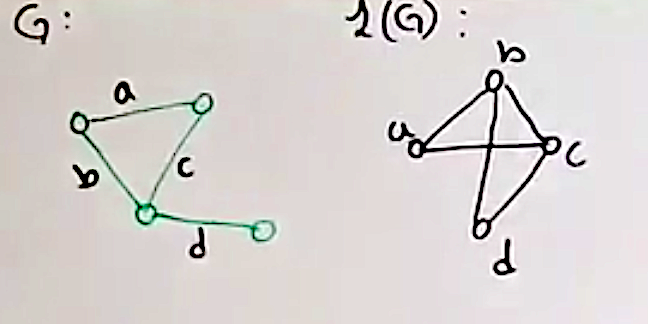
\includegraphics[width=0.45\textwidth]{lineas}
                    \caption{Ejemplo}
                \end{figure}

            %===========+=======================
            % =====       OPERACIONES   ========
            % ==================================
            \subsection{Operaciones}

                \begin{itemize}
                    \item 
                        Si tenemos dos graficas $G, H$ ajenas en vertices entonces definimos a $G \cup H$ como:
                        \begin{itemize}
                            \item $V(G \cup H) = V(G) \cup V(H)$
                            \item $A(G \cup H) = A(G) \cup A(H)$
                        \end{itemize}

                    \item 
                        Si tenemos dos graficas $G, H$ ajenas en vertices entonces definimos a $G + H$ como:
                        \begin{itemize}
                            \item $V(G \cup H) = V(G) \cup V(H)$
                            \item $A(G \cup H) = A(G) \cup A(H) \cup \Set{xy \Such x \in G \text{ y } y \in H}$
                        \end{itemize}

                        Entonces:
                        \begin{itemize}
                            \item $n_{G+H} = n_G + n_H$
                            \item $m_{G+H} = m_G + m_H + n_G n_H$
                        \end{itemize}

                    \item 
                        Si tenemos dos graficas $G, H$ ajenas en vertices entonces definimos a $G \times H$ como:
                        \begin{itemize}
                            \item $V(G \times H) = \Set{x, y \Such x \in G \text{ y } y \ in H} = V(G) \times V(H)$
                            \item $A(G \times H) = \Set{(uv)(xy) \Such x \in G \text{ y } 
                                v = y \text{ y } ux \in A(G) 
                                \text{ o }
                                u = x \text{ y } vy \in A(H) 
                                }$
                        \end{itemize}

                        Entonces:
                        \begin{itemize}
                            \item $n_{G+H} = n_G + n_H$
                            \item $m_{G+H} = m_G + m_H + n_G n_H$
                        \end{itemize}

                        \item 
                        Si tenemos una grafica $G$ y un vertice $v \not \in V(H)$
                        entonces definimos a $G + v$ como:
                        \begin{itemize}
                            \item $V(G + v) = V(G) \cup \Set{v}$
                            \item $A(G + v) = A(G) \cup \Set{xy \Such y \in V(G)}$
                        \end{itemize}

                        \item 
                        Si tenemos una grafica $G$ y un vertice $v\in V(H)$
                        entonces definimos a $G - v$ como:
                        \begin{itemize}
                            \item $V(G - v) = V(G) - \Set{v}$
                            \item $A(G - v) = A(G) - \Set{xv \Such xv[[]] \in A(G)}$
                        \end{itemize}

                        \item [[]]
                        Si tenemos una grafica $G$ y una arista $xy \in A(H)$
                        entonces definimos a $G + xy$ como:
                        \begin{itemize}
                            \item $V(G - v) = V(G) \cup \Set{x, y}$
                            \item $A(G - v) = A(G) \cup \Set{xy}$
                        \end{itemize}

                \end{itemize}
            
            
            %===================================
            % =====   VERTICE DE CORTE     =====
            % ==================================
            \subsection{De Corte}

            Decimos que un vertice $v$ es de corte, si $G-v$ tiene mas componentes de $G$.
            
            Decimos que una arista $xy$ es de corte / un puente si $G-xy$ tiene mas componentes de $G$.


            Nota que una arista de corte puede aumentar el numero de componentes en solo 1, pero un vertice
            de corte puede hacerlo en mucho mas de uno.


            %===================================
            % =====       DISTANCIA        =====
            % ==================================
            \subsection{Distancia}

                La longitud de la trayectoria mas corta entre $v, y$ es llamada la distancia, en dado
                caso de no existir (si no estan en la misma componente conexa) entonces por definicion decimos 
                que es infinita.


            %===================================
            % =====       ARBOL            =====
            % ==================================
            \subsection{Arbol}

                Una grafica $G$ es un arbol si es conexa y ademas no tiene ciclos.
                Decimos que una union de arboles como bosques.
                
                Otra definicion alterna es que toda arista es un puente.


            %===================================
            % =====       BLOQUES          =====
            % ==================================
            \subsection{Bloques}

                Una grafica $G$ es una sub grafica conexa, con el maximo numero de vertices
                y que no tiene vertices de corte. 

            %===================================
            % =====       BLOQUES          =====
            % ==================================
            \subsection{Grafica de bloques}

                Sea $G$ una grafica, $A$ el conjunto de vertices de corte
                y $B$ el conjunto de bloques de $G$.

                \begin{itemize}
                    \item $V(B(G)) = A \cup B$
                    \item $\forall a in A, b \in B \MegaSpace ab \in A(B(G)) \lIff a in B$
                \end{itemize}


        % =====================================================
        % ==========              TEOREMAS            =========
        % =====================================================
        \clearpage
        \section{Teoremas}

            % ==================================
            % =========      SUMA       ========
            % ==================================
            \subsection{Teorema de Suma}

                Sea $G$ un grafo de orden $n$ y tamaño $m$, entonces tenemos que:
                \begin{equation*}
                    2m = \sum_{v \in V}{grado(v)}
                \end{equation*}

                \begin{SmallIndentation}[1em]
                    Idea de la demostración:
                    
                    Dado que cada arista $xy$ incide en $x$ y $y$ por lo que al sumar todos los grados obtenemos cada conexión
                    2 veces.
                \end{SmallIndentation}

                Nota que por lo tanto la suma de los grados de los vertices de la grafica siempre es par.
                Esto nos llega a algo muy importante, en un grafo el numero de vertices de grado impar es par.
                

            % ==================================
            % =========      VERTICES   ========
            % ==================================
            \subsection{Siempre hay dos vertices con grado igual}

                Sea $G$ una gráfica y $V(G)$ sus vertices, entonces existen 2 vertices $v, u$
                tal que $grado(v) = grado(u)$. (Suponiendo que no se valen vertices a ti mismo y no mas de una
                arista entre dos vertices iguales).

                    % ======== DEMOSTRACION ========
                    \begin{SmallIndentation}[1em]
                        \textbf{Demostración}:

                        Va, supongamos que todos son diferentes, entonces crea una sucesión de dichos grados de los
                        vertices.
                        \begin{itemize}
                            \item  $grado(u_1) = 0$
                            \item  $grado(u_2) = 1$
                            \item  $\dots$
                            \item  $grado(u_n) = n - 1$
                        \end{itemize}

                        Entonces el primero lo mas pequeño que puede empezar es en cero, el siguiente
                        no puede ser cero porque entonces ya valio, asi que si queremos minimizar tiene que ser
                        uno, y asi, entonces en una grafica con $n$ vertices tenemos que el vertices con grado 
                        mayor es $n - 1$, pero piensa que significa que un vertice tenga $n - 1$ aristas, pues
                        que esta conectado a todos los demas.

                        Pero eso no puede ser porque dijimos que $grado(u_1) = 1$, y es mas el grado no puede ser
                        mayor a $n - 1$ porque no hay mas vertices para hacer conexión.


                    \end{SmallIndentation}

                Como comentario, podemos ver el teorema como que siempre hay dos vertices con el mismo grafo
                con el mismo grado.


            % ==================================
            % =========      MAX TAMAÑO ========
            % ==================================
            \subsection{Máximo tamaño}

                Sea $G$ una gráfica simple entonces pasa que:
                \begin{equation*}
                    num_{aristas} = {num_{vertices} \choose 2}
                \end{equation*}
                

                % ======== DEMOSTRACION ========
                \begin{SmallIndentation}[1em]
                    \textbf{Demostración}:

                    
                    \begin{align*}
                        2m
                            &= \sum_{v \in V}{grado(v)}
                                && \Remember{Recuerda que el grado maximo de un vertice es $n -1$}    \\
                            &\leq n (n - 1)
                                && \Remember{por ser el universo}    \\
                            m &\leq \frac{n (n - 1)}{2} \\
                            m &\leq {n \choose 2}
                        \end{align*}


                \end{SmallIndentation}

            % ==================================
            % ====  CAMINO IMPLICA TRAYECTORIA =
            % ==================================
            \subsection{Camino implica trayectoria}

                Para todo $uv$-camino hay una $uv$-trayectoria.

            % ==================================
            % ====  CAMINO IMPLICA TRAYECTORIA =
            % ==================================
            \subsection{Camino y ciclos}

                Si tenemos un camino cerrado de longitud impar 
                entonces existe un ciclo de longitud impar.

            % ==================================
            % ====  CAMINO IMPLICA TRAYECTORIA =
            % ==================================
            \subsection{Ciclos y trayectorias}

                Todo ciclo tiene exactamente dos trayectorias independientes entre cualquiera
                dos verticesbu.

                Toda graficca bipartita no tiene ciclos impares.


            % ==================================
            % =========     CONEXAS      =======
            % ==================================
            \subsection{Conexas}

                \begin{itemize}
                    \item Sea $G$ una grafica conexa de orden $n$ y tamano $m$, si $n \geq 2$ entonces $m \geq n - 1$
                \end{itemize}

            % ==================================
            % ======    BIPARTITAS       =======
            % ==================================
            \subsection{Bipartitas}

                \begin{itemize}
                    \item Sea $G$ una grafica conexa, entonces $G$ 
                    es bipartita si y solo si no tiene ciclos de longitud impar.

                    Podemos ver como un colorario random que todo arbol es una grafica bipartita
                \end{itemize}


            % ==================================
            % =========     ARBOLES      =======
            % ==================================
            \subsection{Arboles}

                \begin{itemize}
                    \item Para un arbol de orden $n$ hay $m = n - 1$
                    \item Una grafica es un arbol si y solo si existe un unico camino entre cuales quiera dos vertices
                    \item Tienen al menos dos vertices de grado 1.
                    \item Si le quitas una hoja a un arbol, la grafica resultante sigue siendo un arbol
                    \item Sea $G$ una grafica conexa de orden $n$ entonces:
                    \begin{itemize}
                        \item G es arbol, es decir sin ciclos y conexa
                        \item G no tiene ciclos y tiene $n - 1$ aristas
                        \item G es conexa y tiene $n - 1$ aristas
                    \end{itemize}

                    \item Sea $G$ una grafica conexa entonces contiene un arbol generador
            \end{itemize}
                


            % ==================================
            % =========     CONEXIDAD    =======
            % ==================================
            \subsection{Conexidad}

                \begin{itemize}
                    \item Si se tiene un puente tiene un vertice de corte
                    \item $v$ es de corte si y solo si, para toda trayectoria entre dos vertices cuales quiera
                    de dos componentes todas sus trayectorias pasan por ese vertice
                    \item Sea $G$ una grafica 3-regular entonces tiene un vertice de corte si y solo si 
                    tiene un puente
                \end{itemize}



\end{document}